\chapter{Results}

The chapter results shows visual results of the three algorithm. Each algorithm was tested with three different images. The images have the following properties:


\begin{table}[H]
    \centering
    \begin{tabular}{|l|l|l|l|}
        \hline
        \textbf{}   & \textbf{dice.png} & \textbf{dice\_large.png} & \textbf{pnglogo-blk.png} \\ \hhline{|=|=|=|=|}
        Width       & 800px             & 1754px                   & 1024px                   \\ \hline
        Height      & 600px             & 1554px                   & 768px                    \\ \hline
        Filesize    & 295 KB            & 1.5 MB                   & 516                      \\ \hline
        Transparent & No                & Yes                      & No                       \\ \hline
    \end{tabular}
\end{table}

In the following sections the first image row is always the \textbf{dice.png}, the second image row is the \textbf{dice\_large.png} and the third row always shows the \textbf{pnglogo-blk.png}.\\

The x-axis of each plot shows the number of threads used and the y-axis shows the execution time in ms of the corresponding variant.

\newpage
\section{Grayscale}

The self-implemtend version yielded exactly the same visual results as the OpenCV version wich was expected because the same formular was used.

\begin{figure}[H]
    \centering

    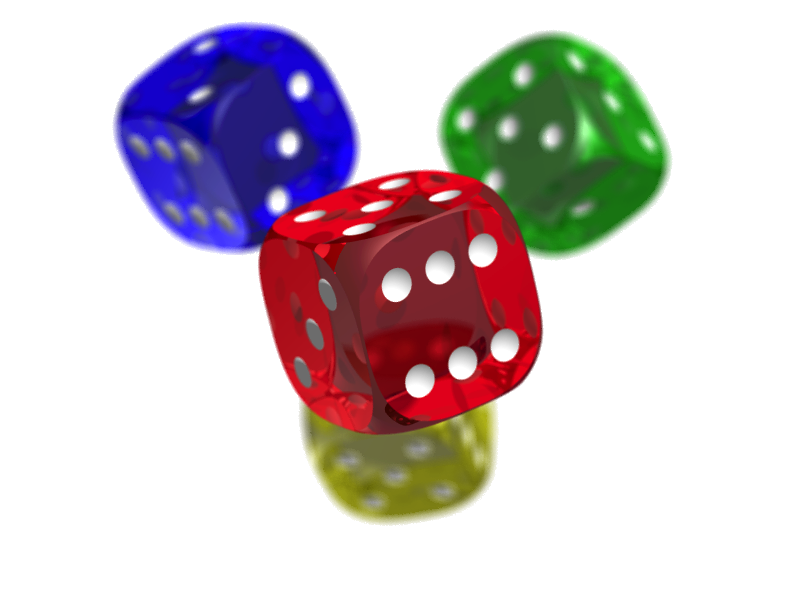
\includegraphics[width=0.30\textwidth]{images/dice.png}
    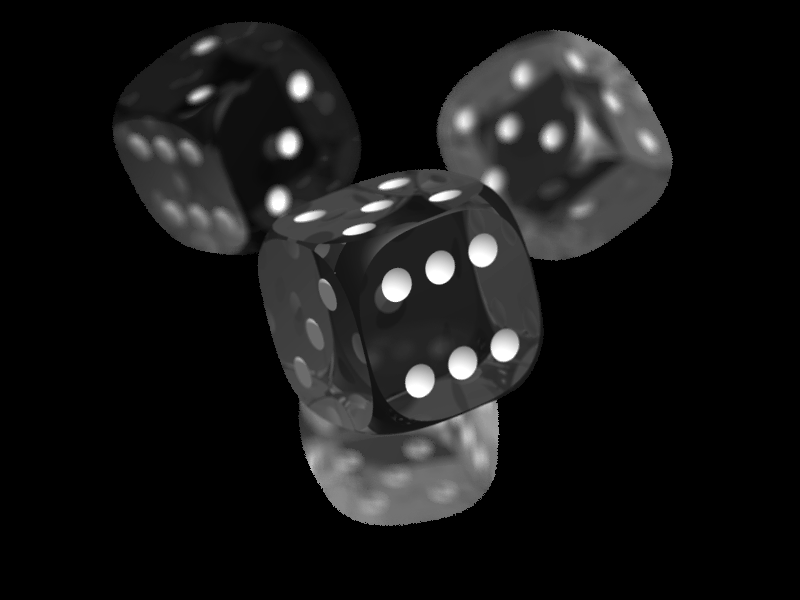
\includegraphics[width=0.30\textwidth]{images/results/grayscale-cv.dice.png}
    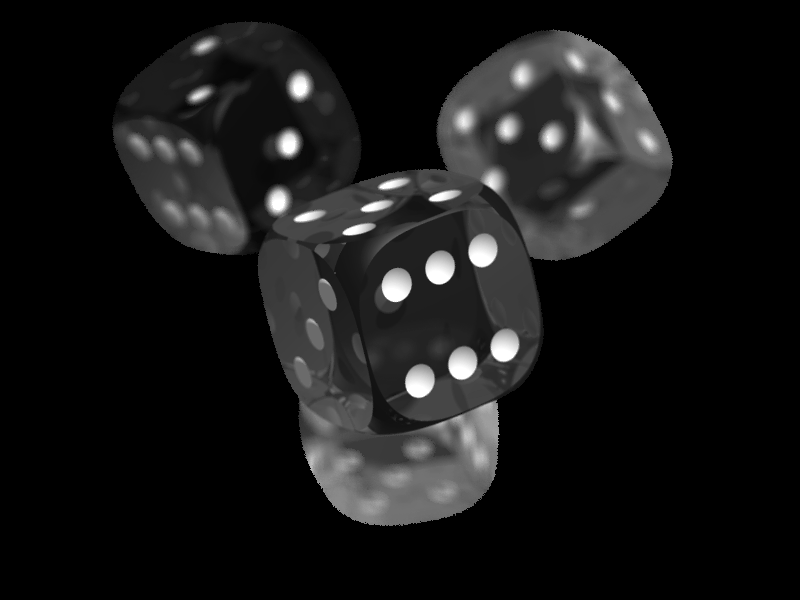
\includegraphics[width=0.30\textwidth]{images/results/grayscale-my.dice.png}
    \\
    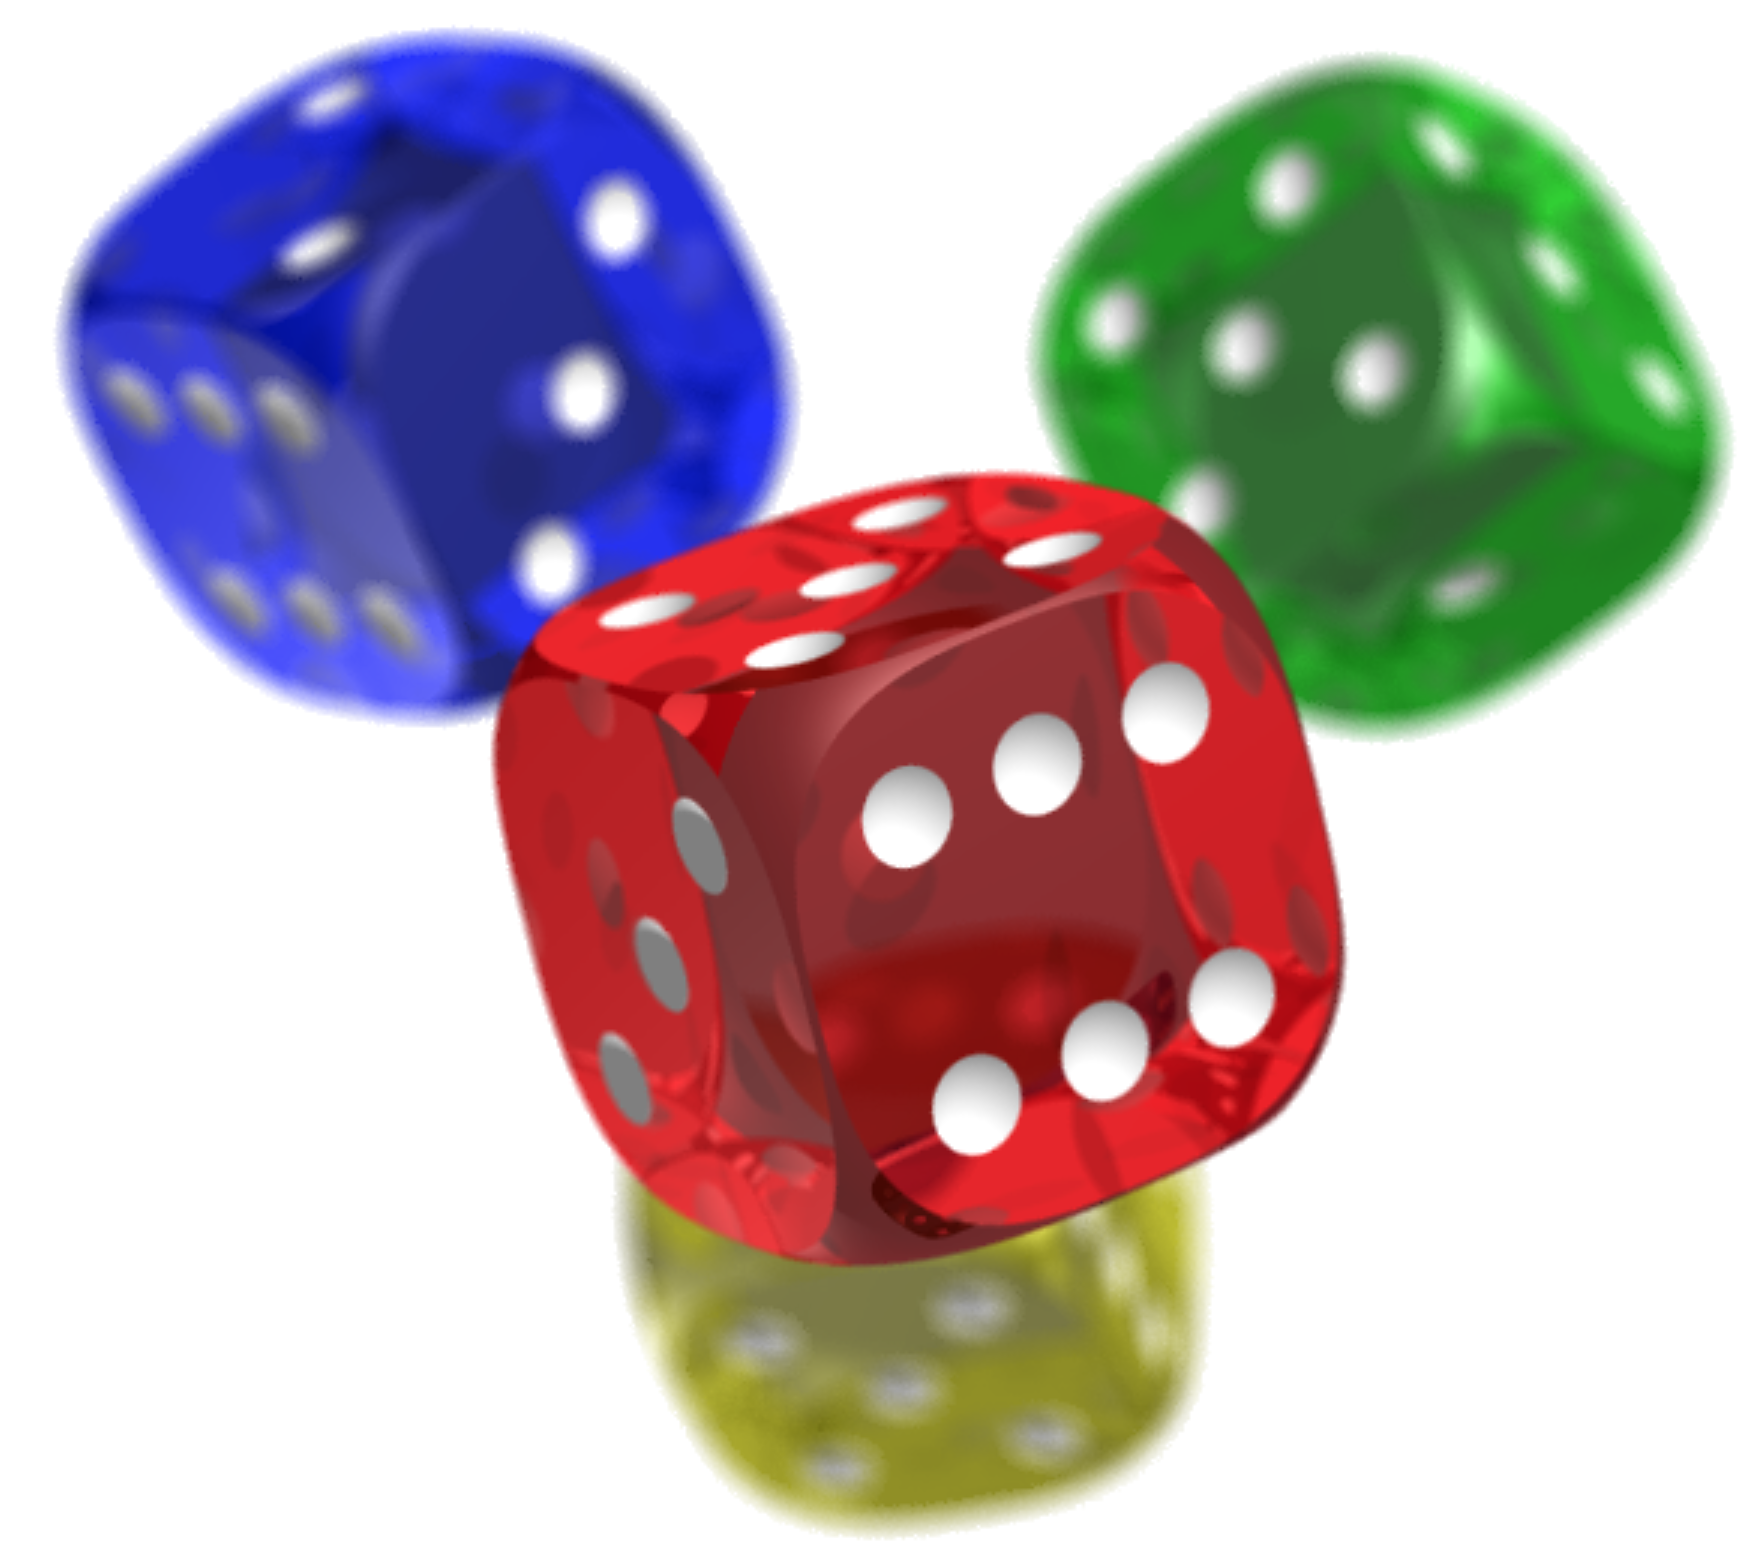
\includegraphics[width=0.30\textwidth]{images/dice_large.png}
    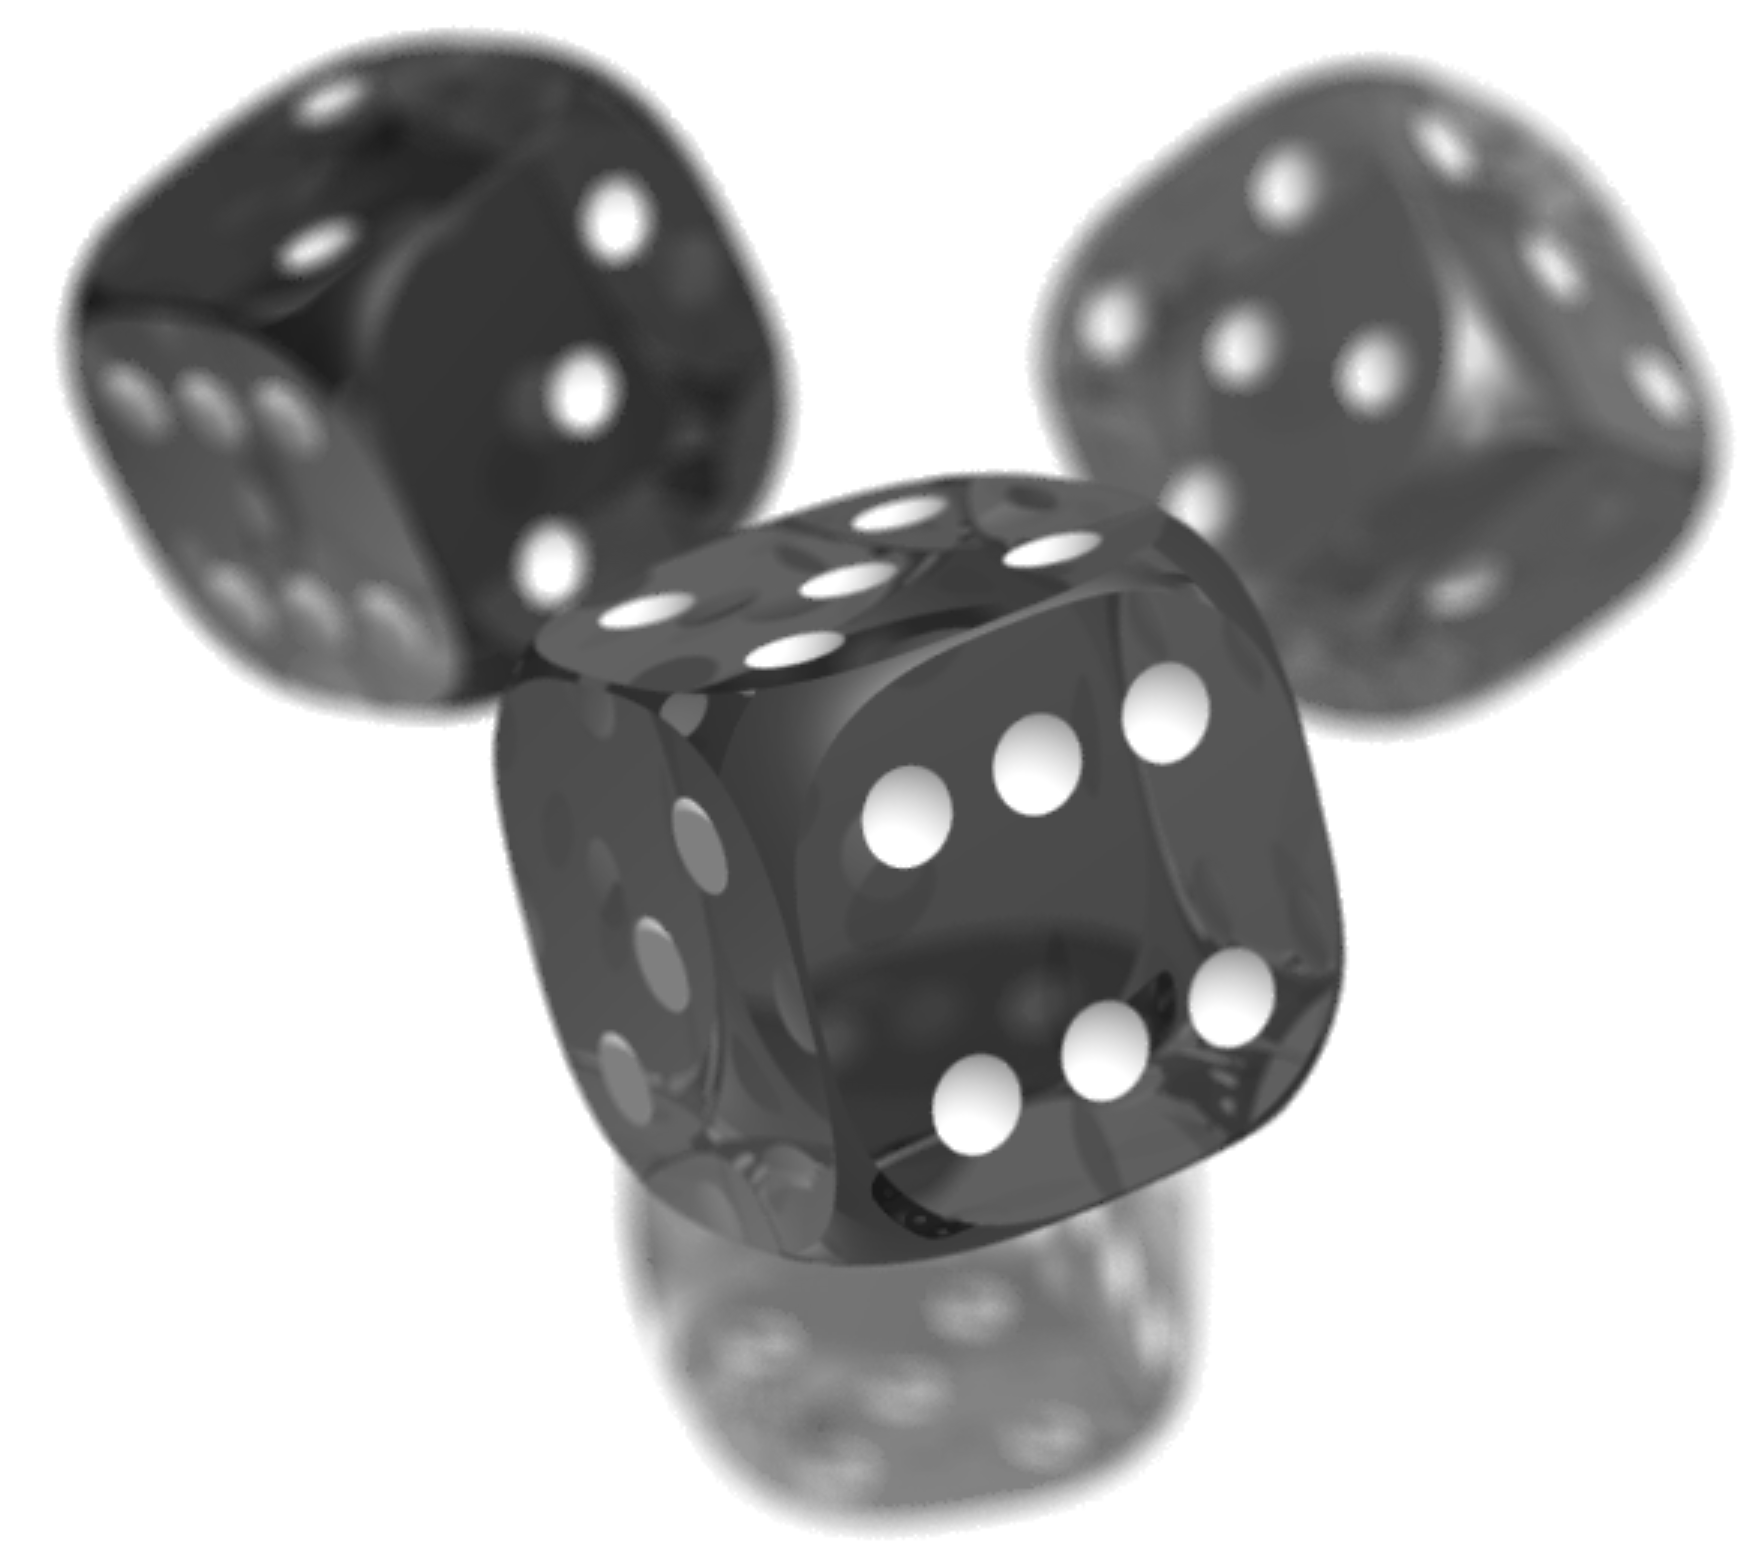
\includegraphics[width=0.30\textwidth]{images/results/grayscale-cv.dice_large.png}
    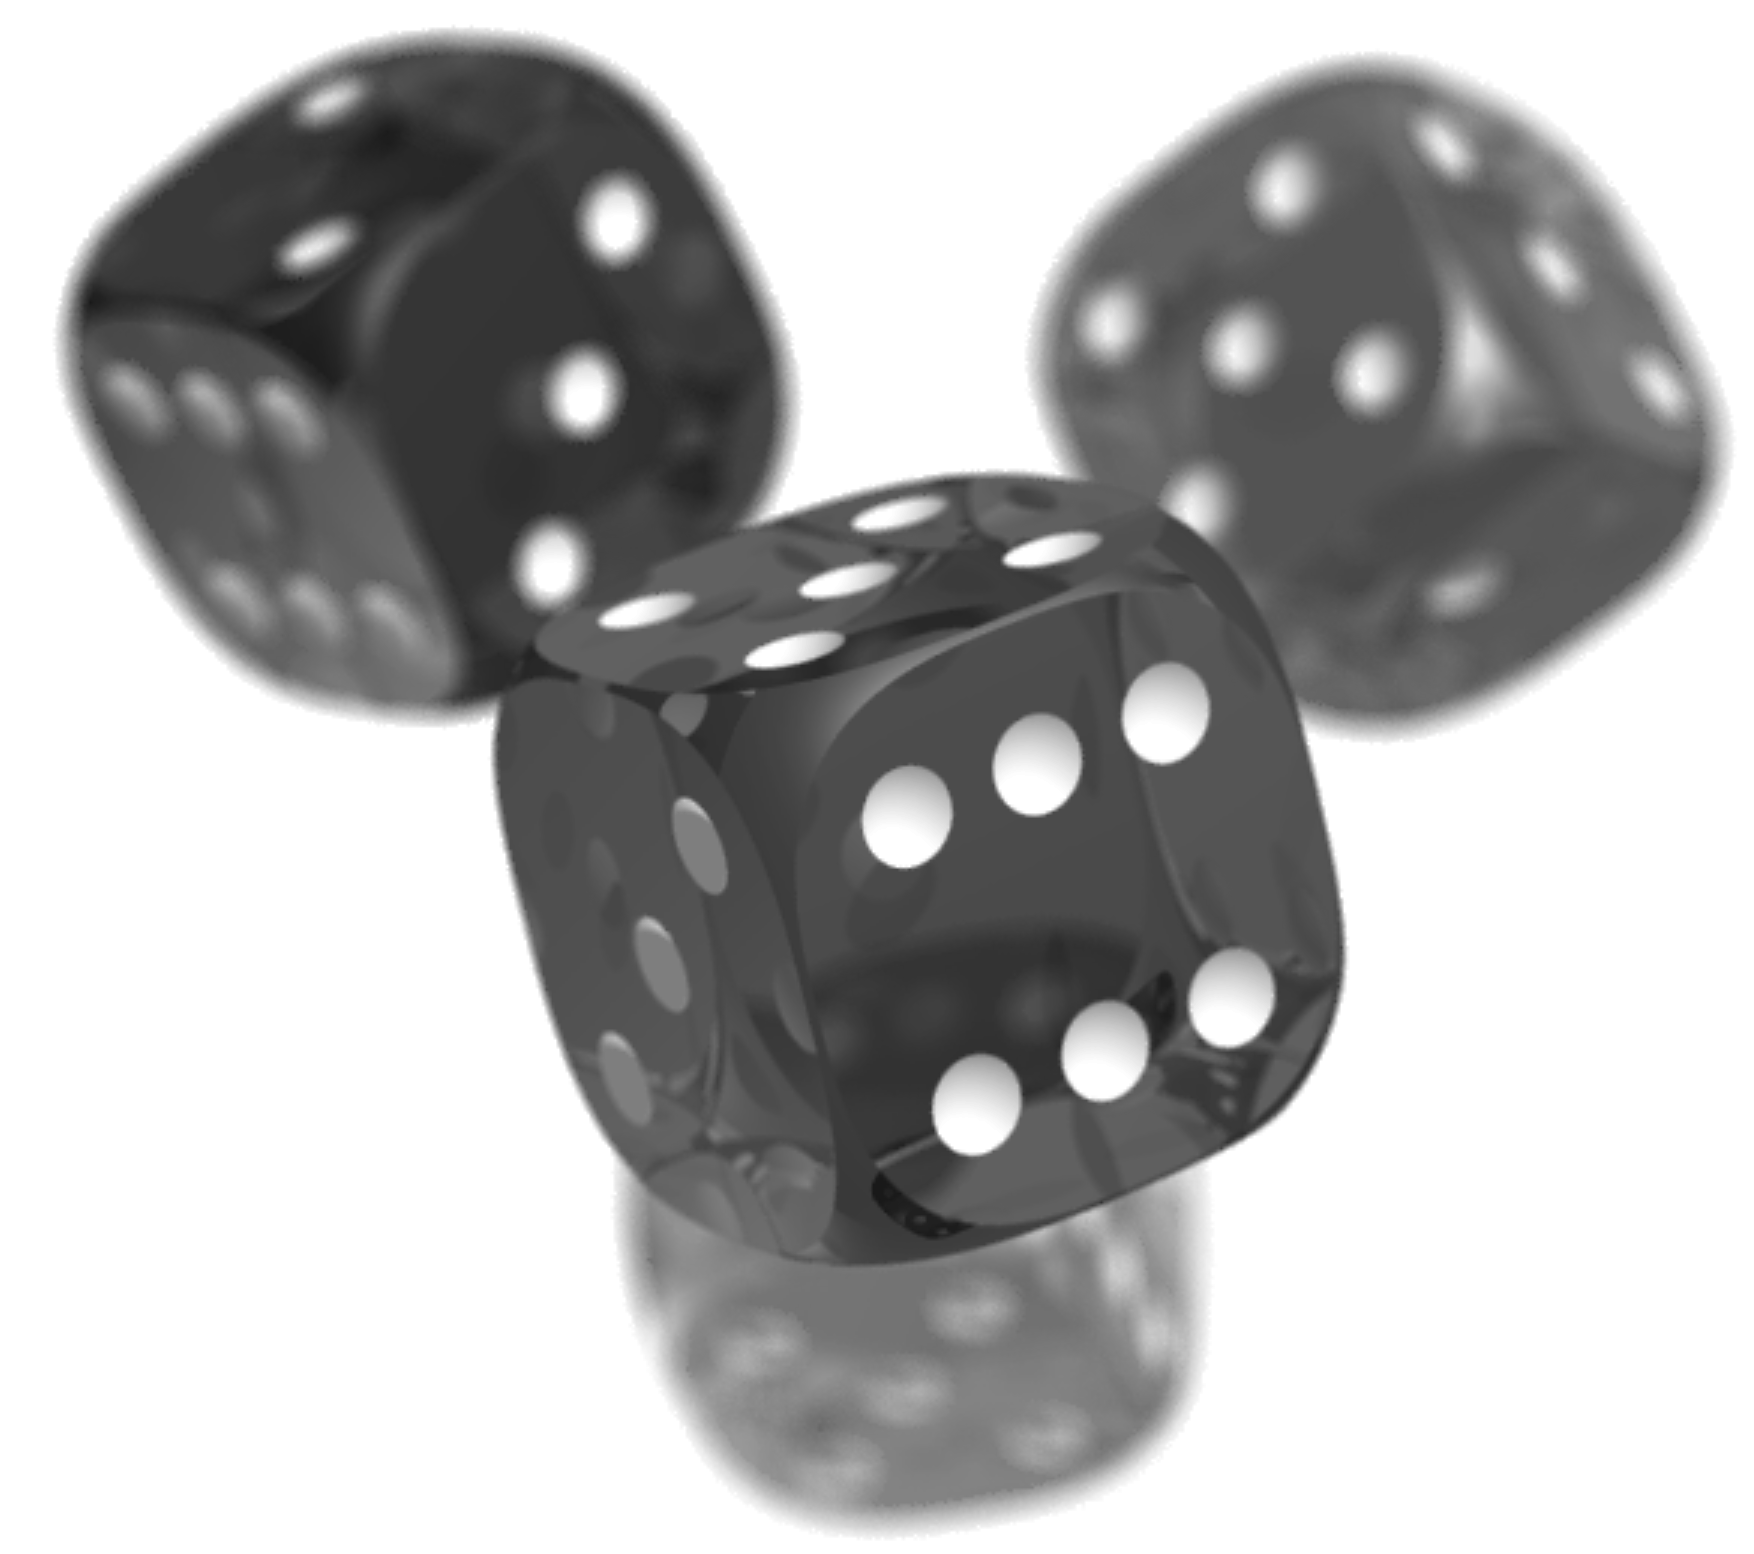
\includegraphics[width=0.30\textwidth]{images/results/grayscale-my.dice_large.png}
    \\
    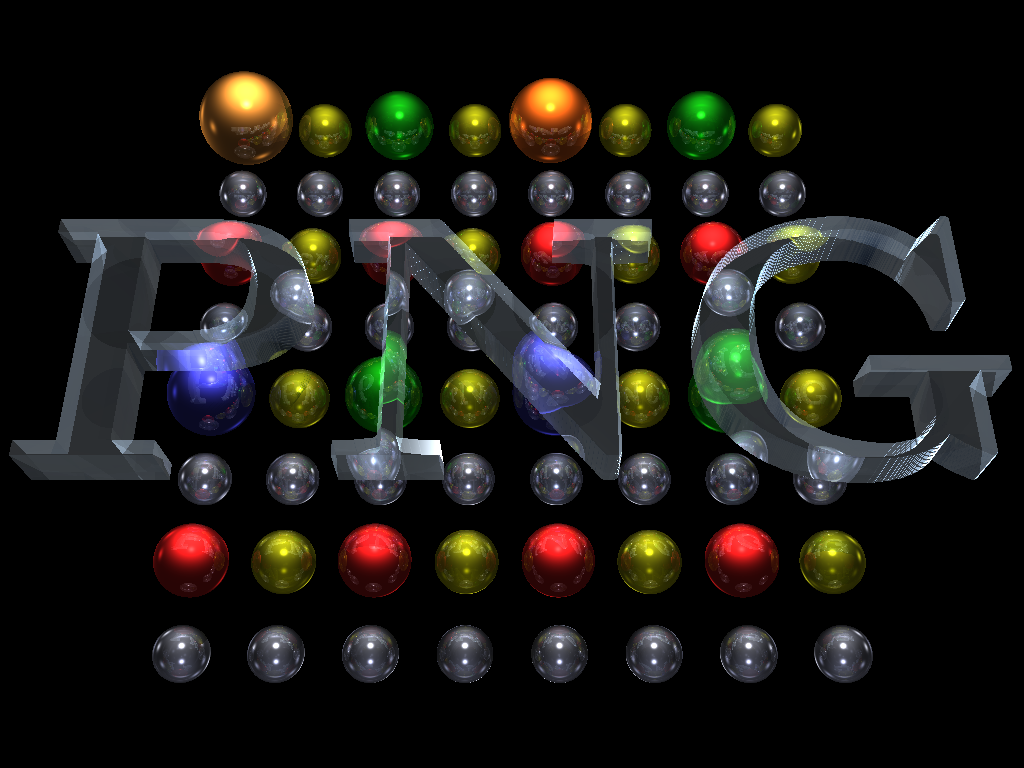
\includegraphics[width=0.30\textwidth]{images/pnglogo-blk.png}
    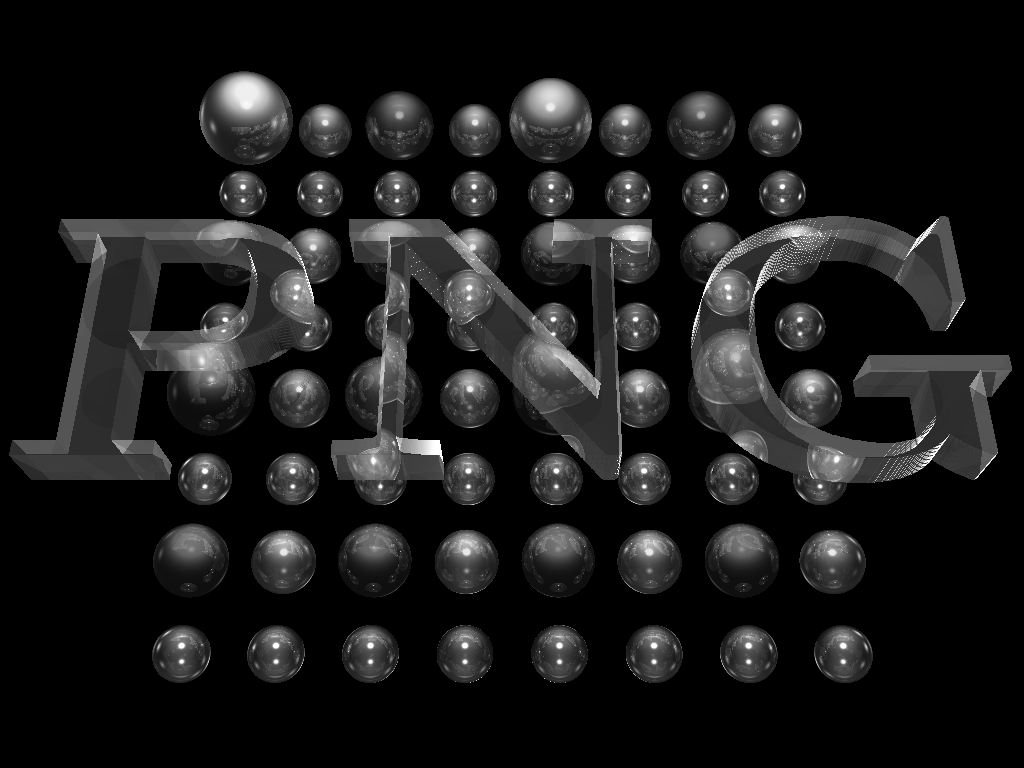
\includegraphics[width=0.30\textwidth]{images/results/grayscale-cv.pnglogo-blk.png}
    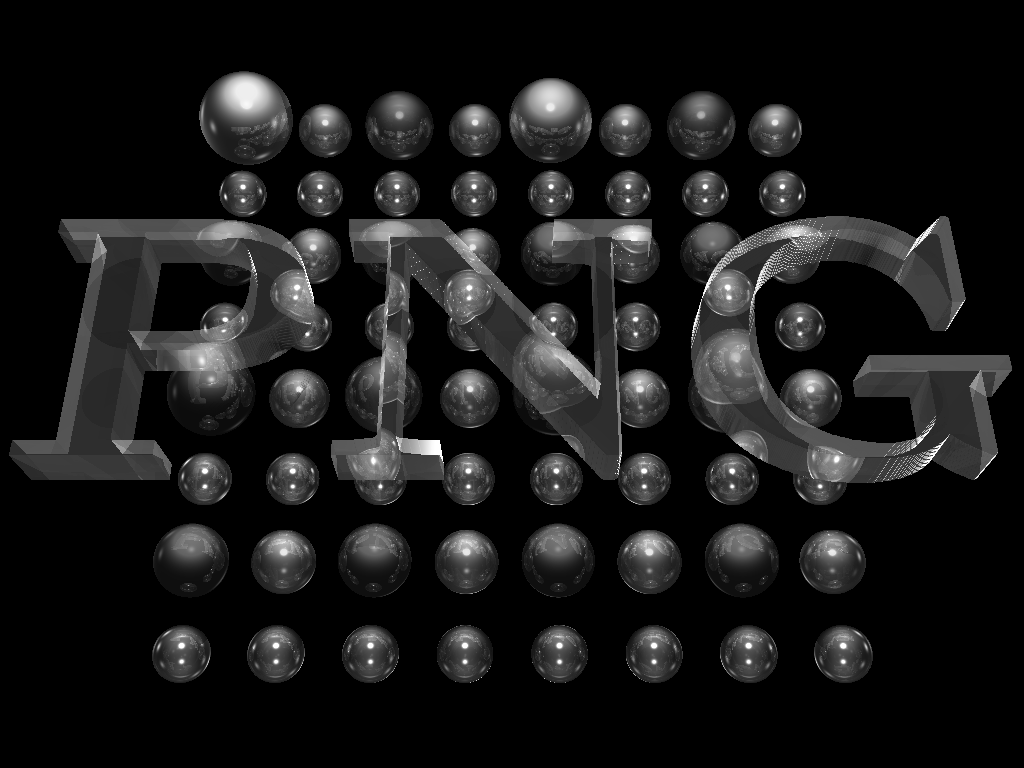
\includegraphics[width=0.30\textwidth]{images/results/grayscale-my.pnglogo-blk.png}

    \begin{center}
        \caption{Grayscale results of OpenCV (middle) and self-implemented  Algorithm (right)}            
    \end{center}

    \label{fig:grayscale1}
\end{figure}

The top performance results for grayscale were $ 0.6077 $ ms, $ 9.51975 $ ms  and $ 5.41915 $ ms for the three images. In comparison OpenCV took $ 0.0876 $ ms, $ 0.5389 $ ms and $ 0.14725 $ ms.


\begin{center}
    \begin{figure}[H]
        \centering
        \begin{center}
    \begin{figure}[H]
        \centering

        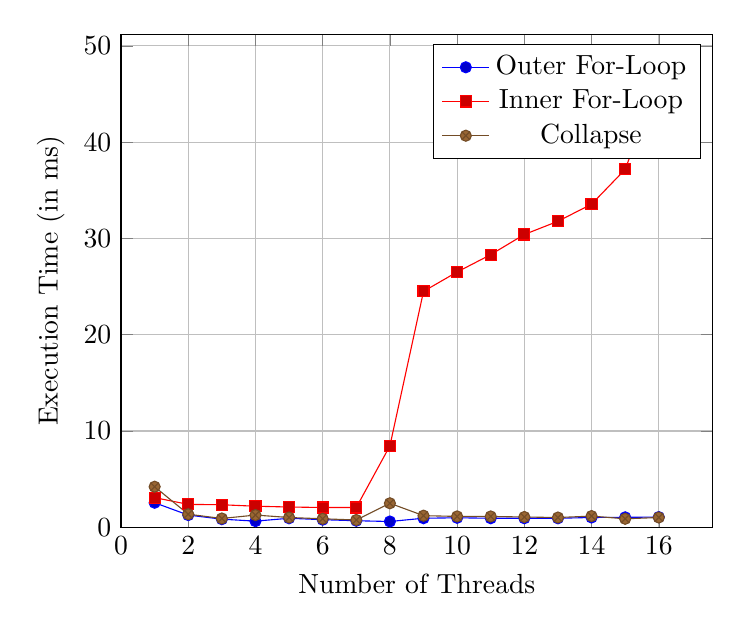
\begin{tikzpicture}
            \begin{axis}[
                title={},
                width=0.75\textwidth,
                xlabel={Number of Threads},
                ylabel={Execution Time (in ms)},
                xmin=0,
                ymin=0,
                grid=major
            ]
                \addplot coordinates {
                    (1,2.5549)(2,1.2735)(3,0.85025)(4,0.6436)(5,0.94375)(6,0.7966)(7,0.6854)(8,0.6077)(9,0.9472)(10,0.99225)(11,0.9471)(12,0.94635)(13,0.94125)(14,1.02495)(15,1.041)(16,1.06755)
                };
                \addlegendentry{Outer For-Loop}

                \addplot coordinates {
                    (1,3.08615)(2,2.3858)(3,2.34615)(4,2.19415)(5,2.1119)(6,2.0609)(7,2.06245)(8,8.4643)(9,24.5043)(10,26.5145)(11,28.3157)(12,30.4109)(13,31.7816)(14,33.5549)(15,37.1696)(16,46.544)
                };
                \addlegendentry{Inner For-Loop}       

                \addplot coordinates {
                    (1,4.2187)(2,1.36355)(3,0.92205)(4,1.27645)(5,1.0218)(6,0.8902)(7,0.76425)(8,2.5011)(9,1.21405)(10,1.13565)(11,1.1338)(12,1.0742)(13,1.0206)(14,1.17005)(15,0.88735)(16,1.0243)
                };
                \addlegendentry{Collapse}
            \end{axis}
        \end{tikzpicture}
        \caption{Grayscale Performance Tests dice.png}
    \end{figure}
\end{center}
        \caption{Performance results of Grayscale conversion algorithm}
    \end{figure}
\end{center}

\newpage
\section{HSV}

The self-implemented version of the HSV algorithm yielded slightly different results compared with the OpenCV version. By substracting the two resulting image matrices, it showed small error values. These differences are not visible by eye and could be the result of different floating number rouding behaviour.

\begin{figure}[H]
    \centering

    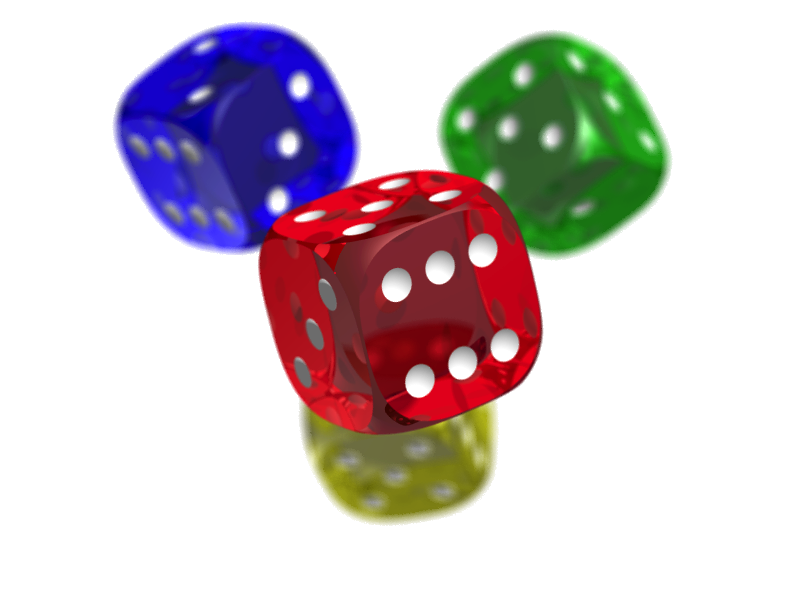
\includegraphics[width=0.30\textwidth]{images/dice.png}
    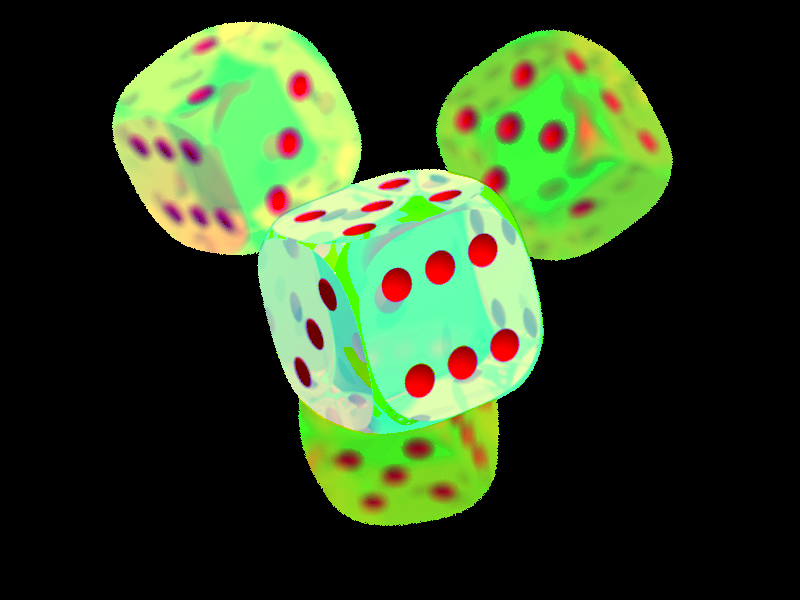
\includegraphics[width=0.30\textwidth]{images/results/hsv-cv.dice.png}
    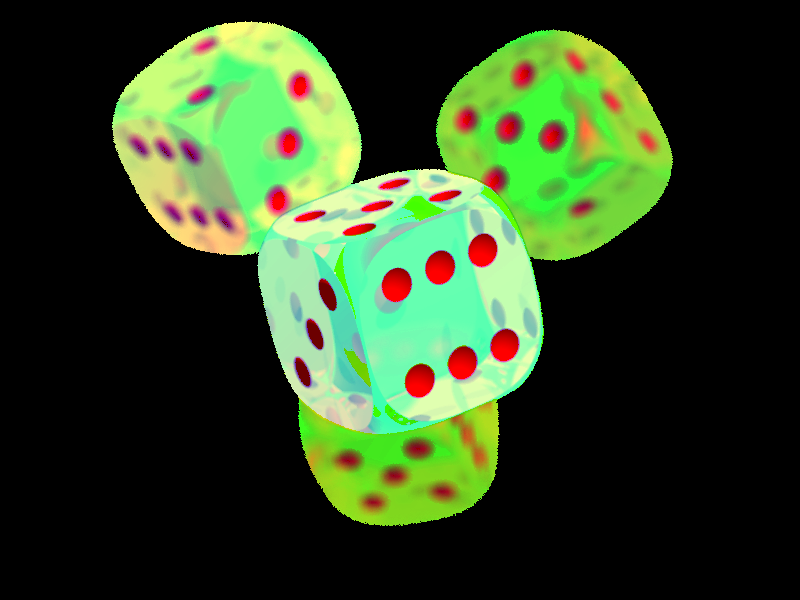
\includegraphics[width=0.30\textwidth]{images/results/hsv-my.dice.png}
    \\
    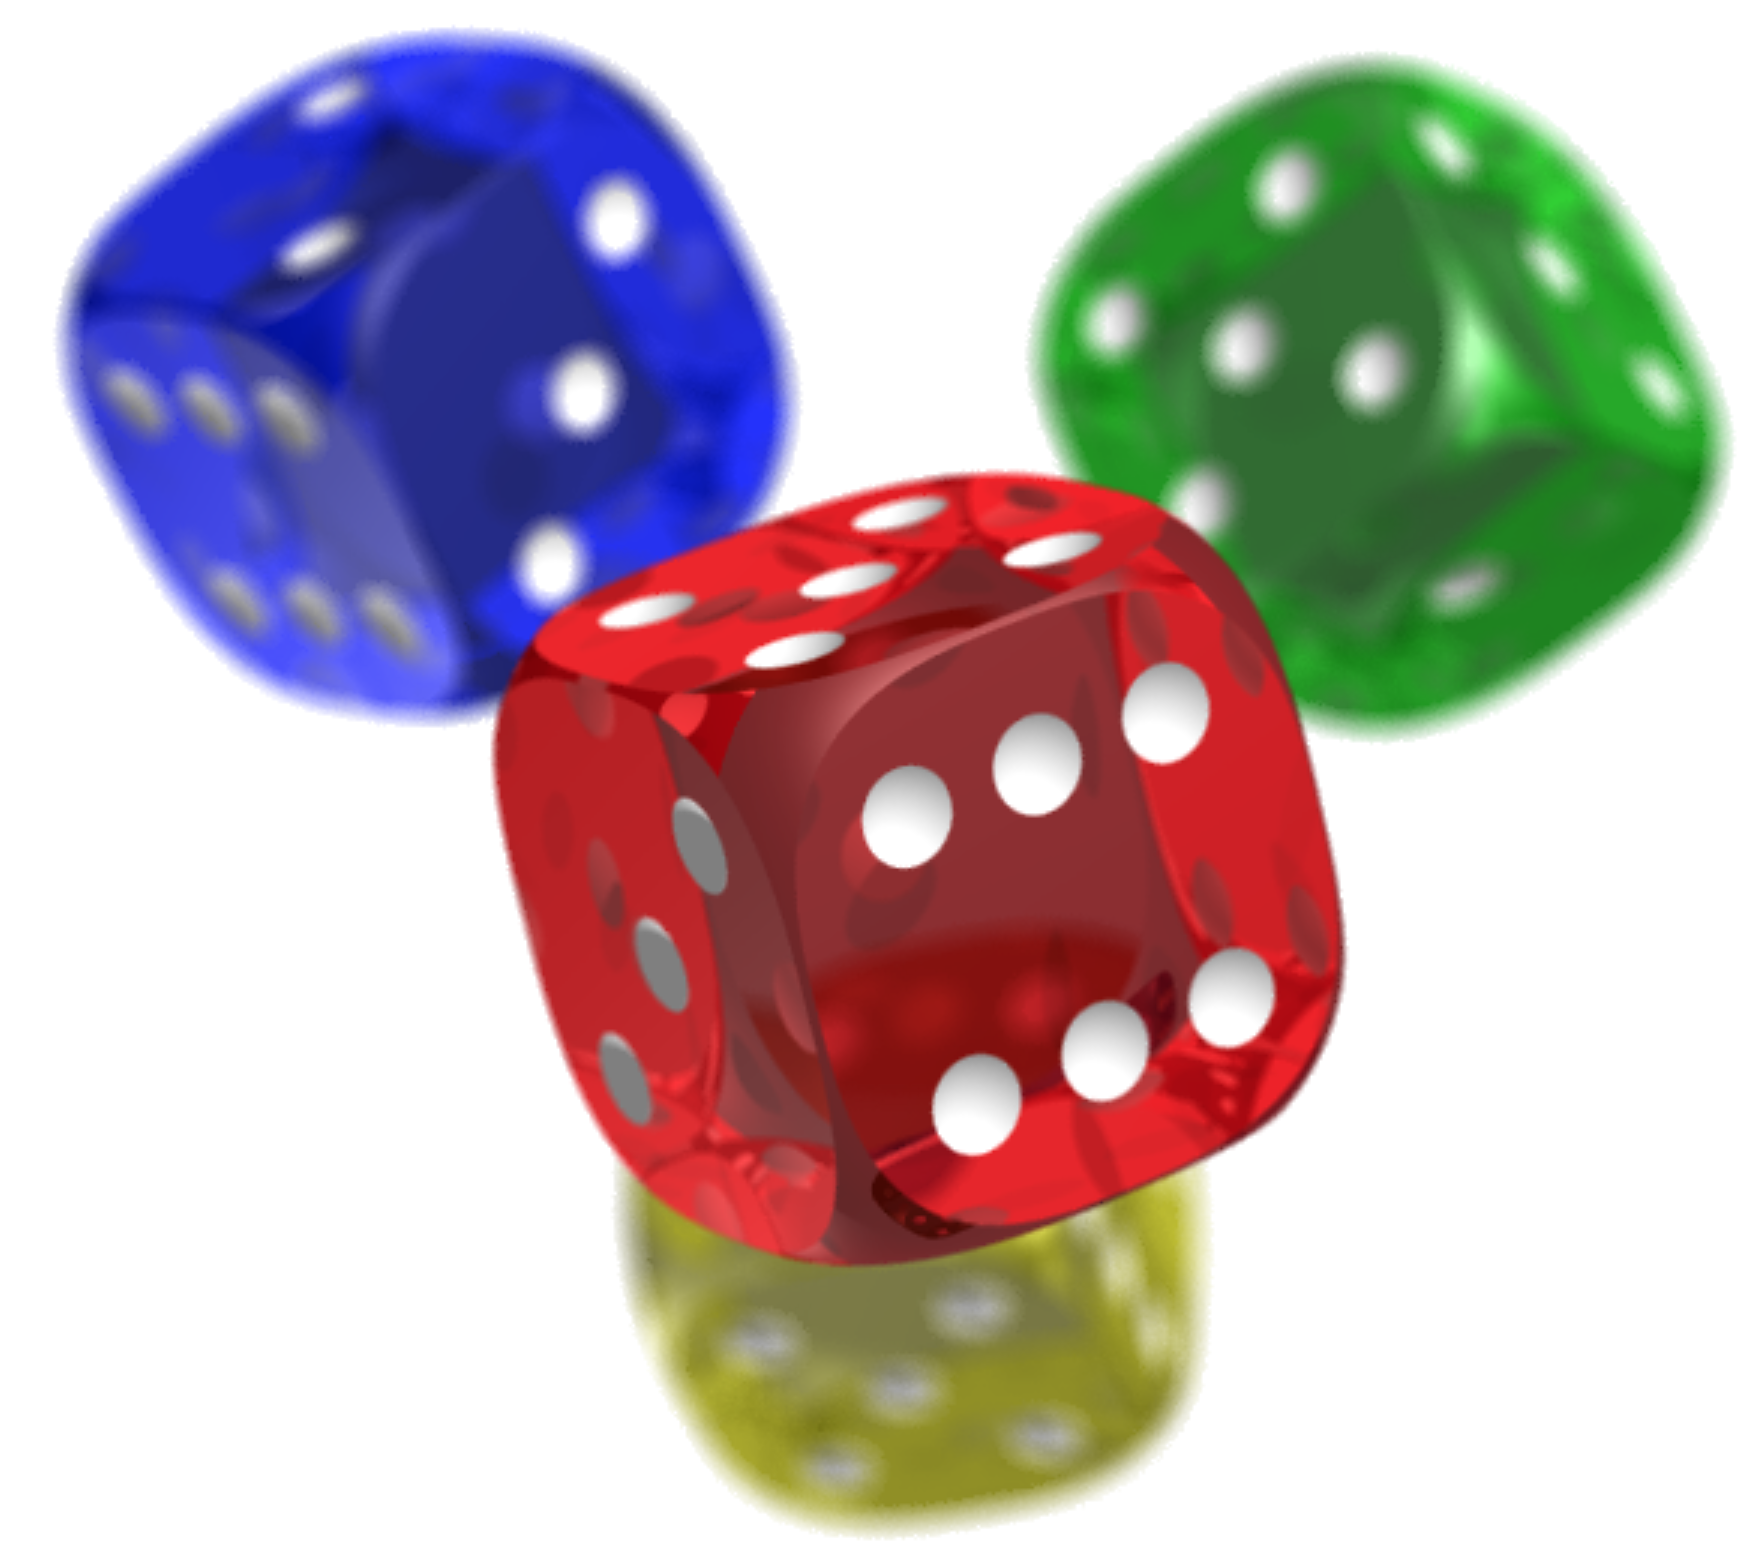
\includegraphics[width=0.30\textwidth]{images/dice_large.png}
    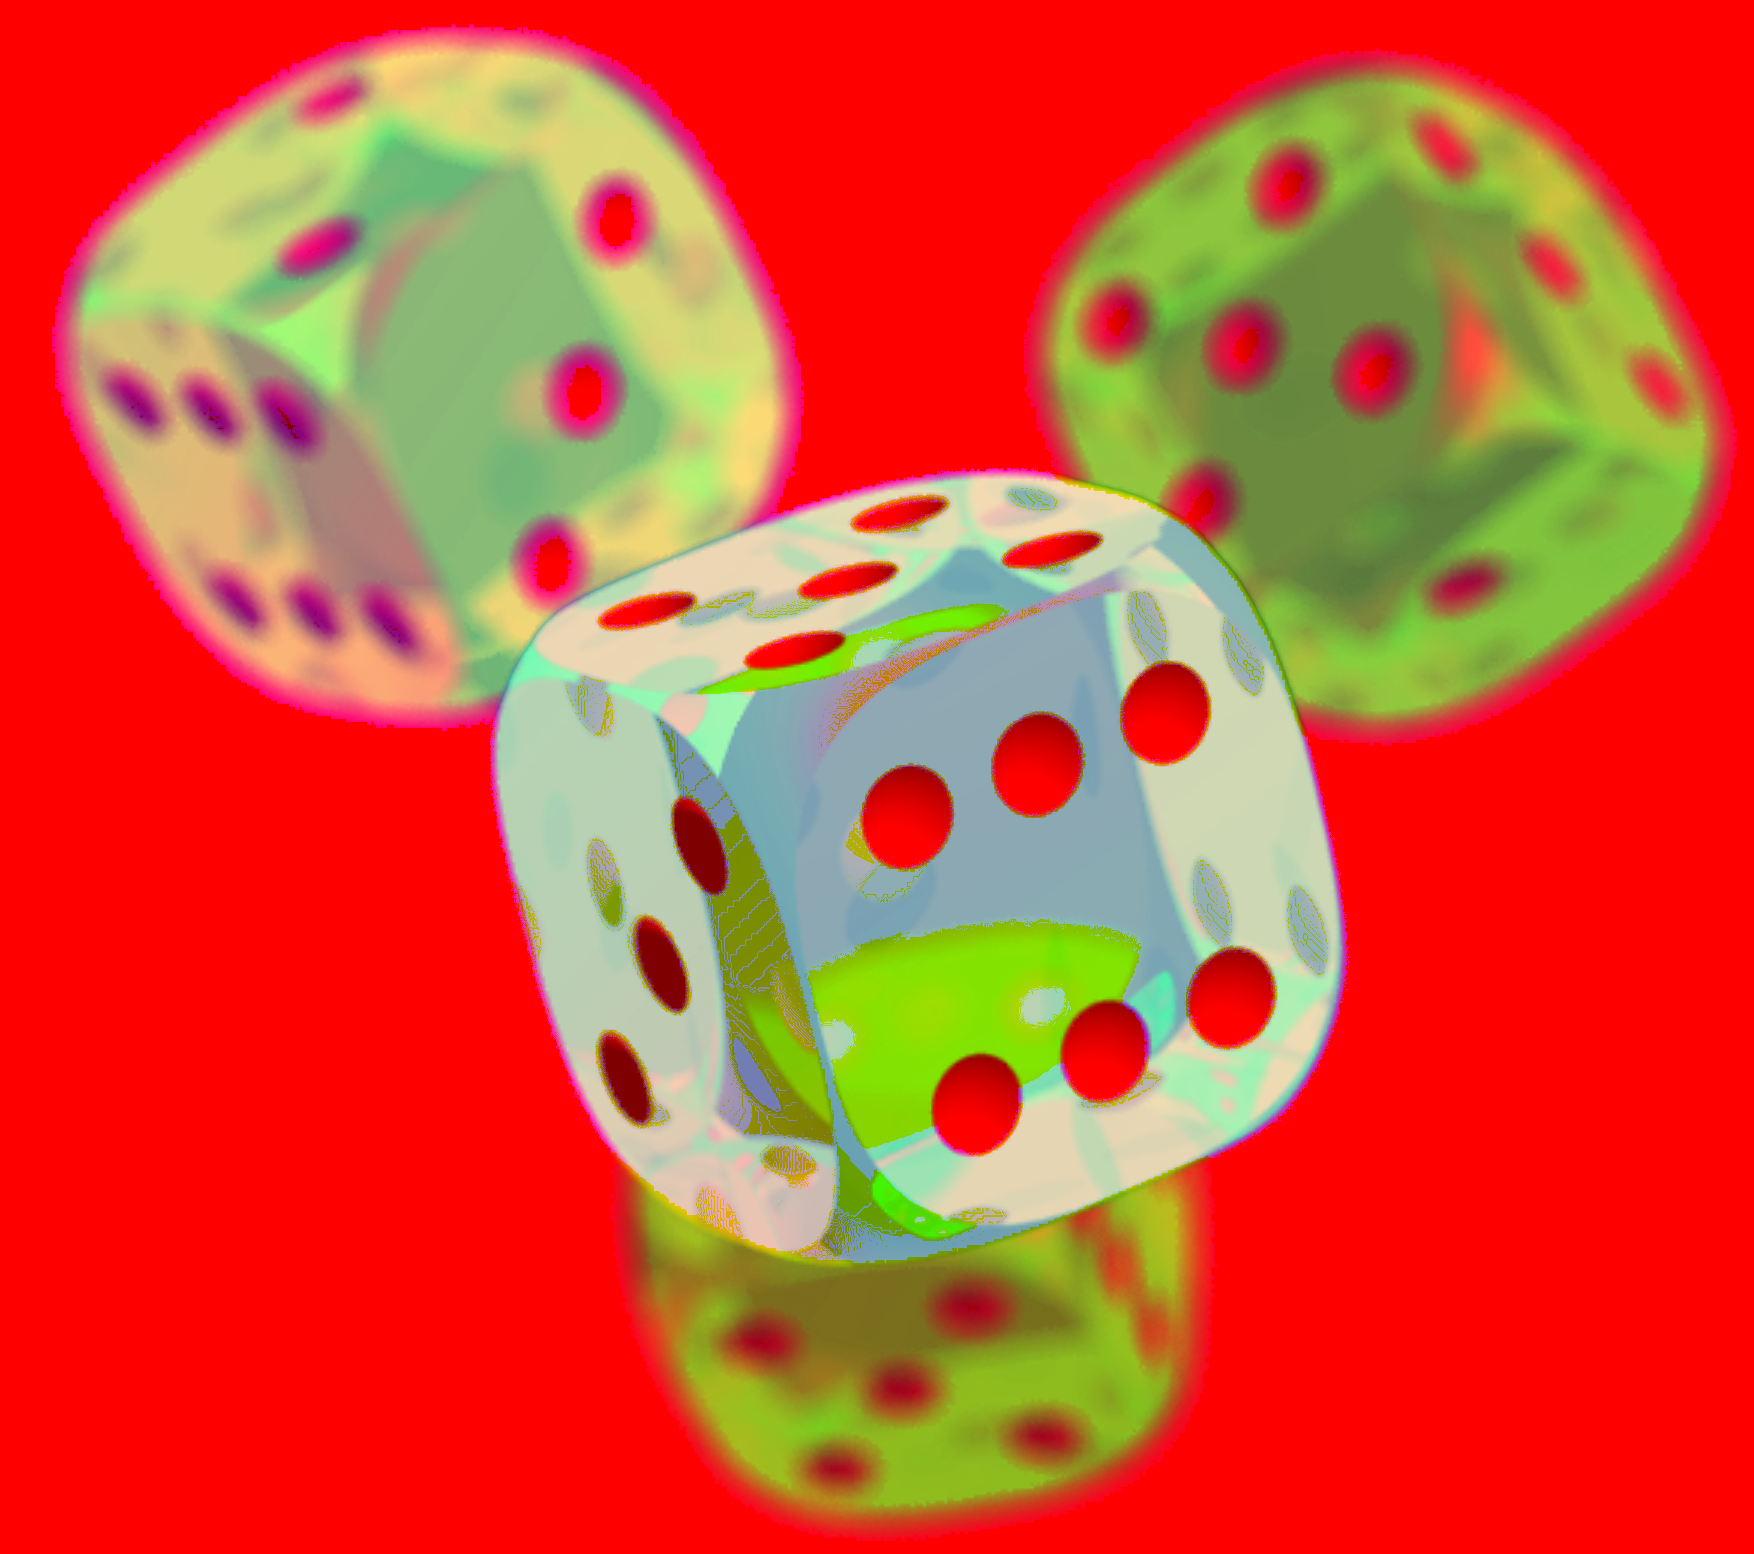
\includegraphics[width=0.30\textwidth]{images/results/hsv-cv.dice_large.png}
    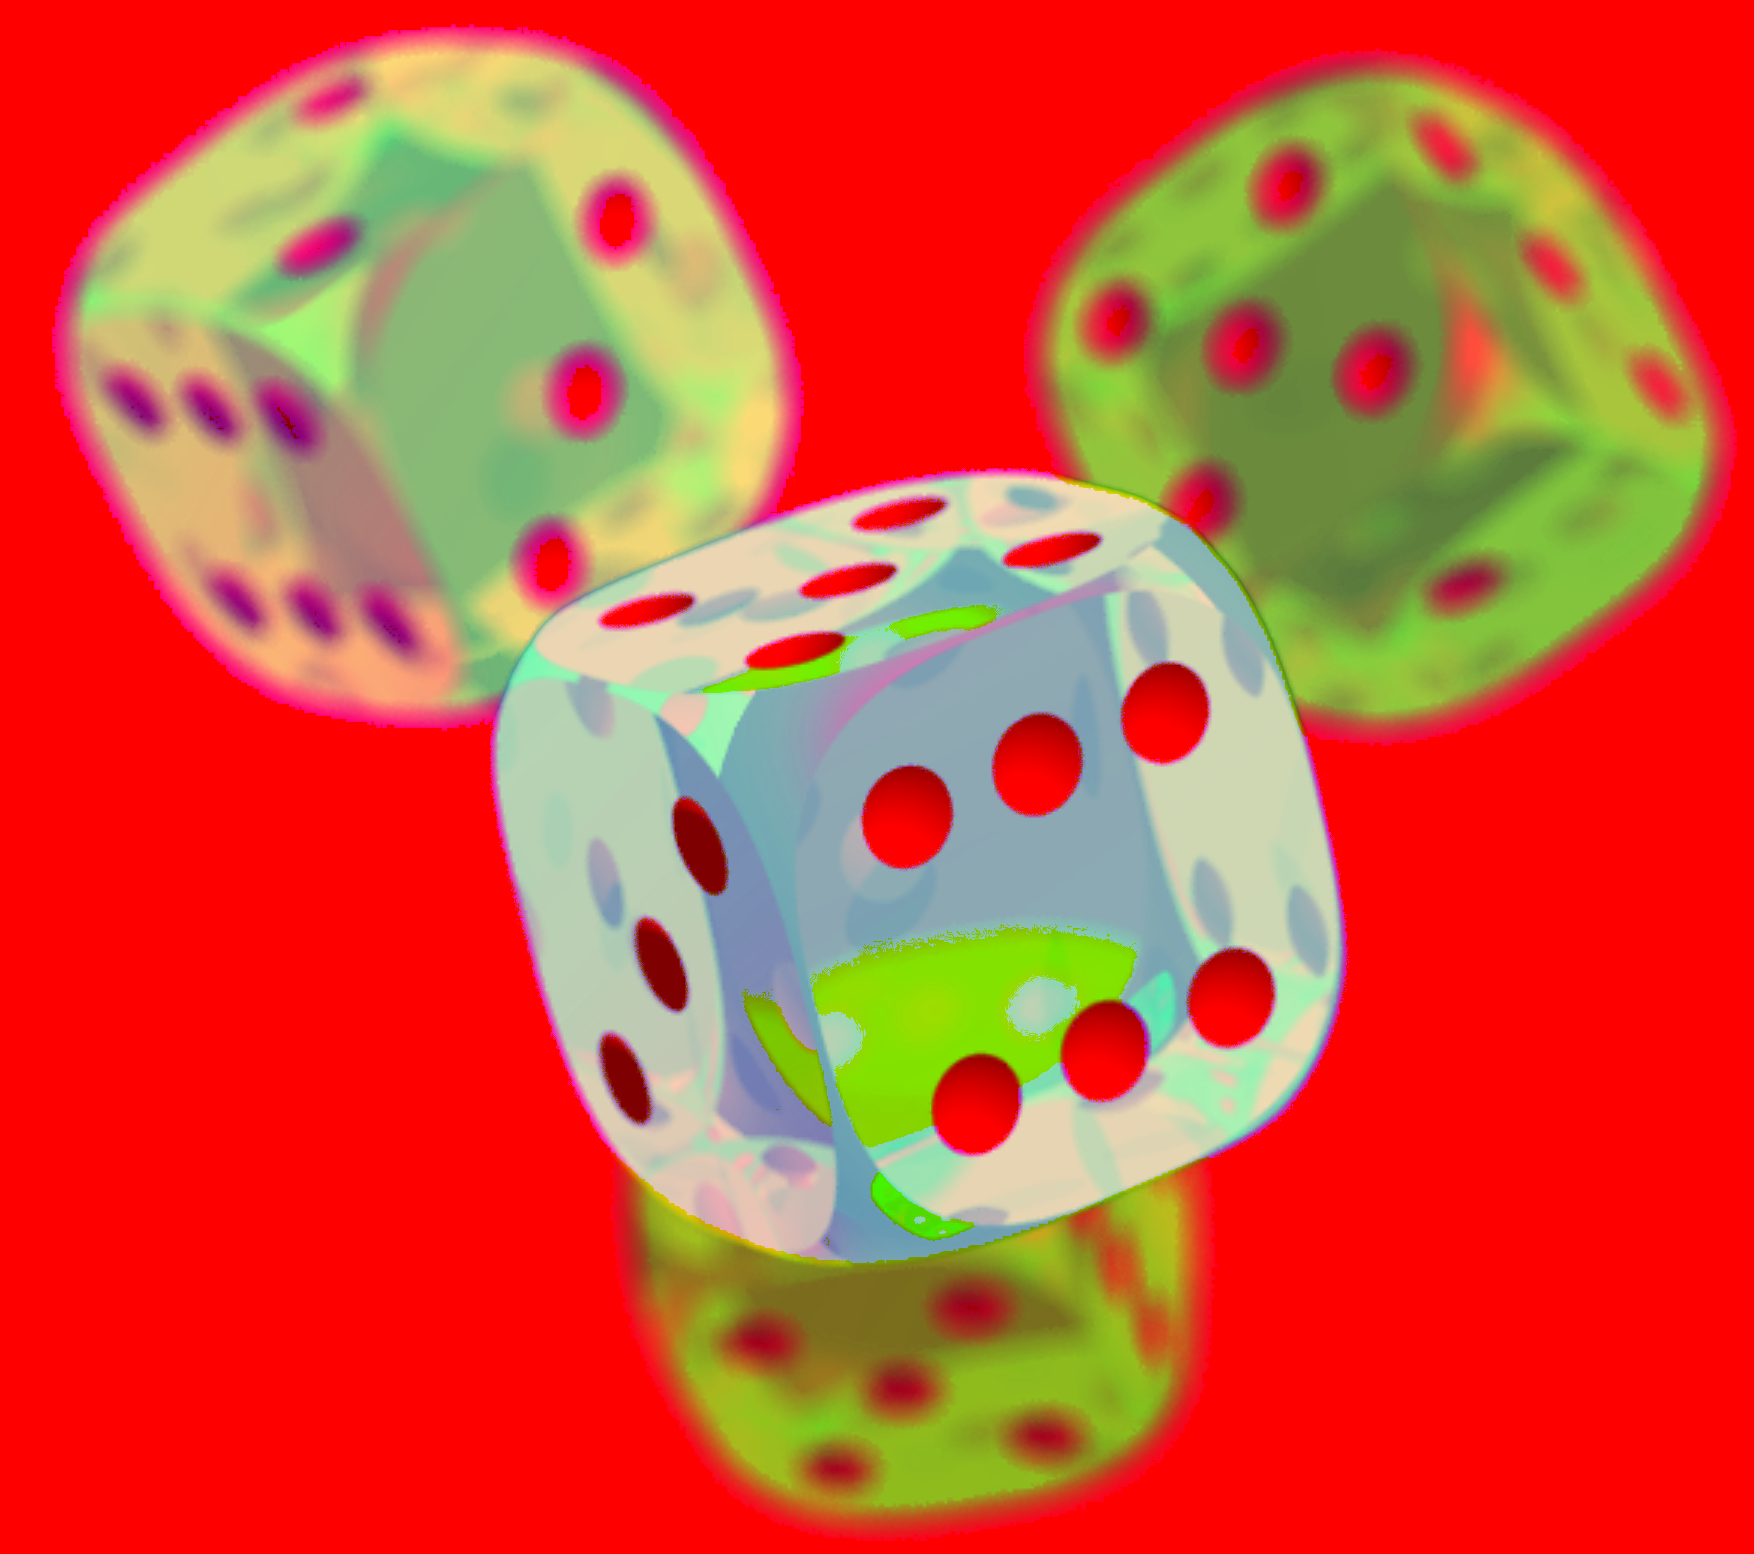
\includegraphics[width=0.30\textwidth]{images/results/hsv-my.dice_large.png}
    \\
    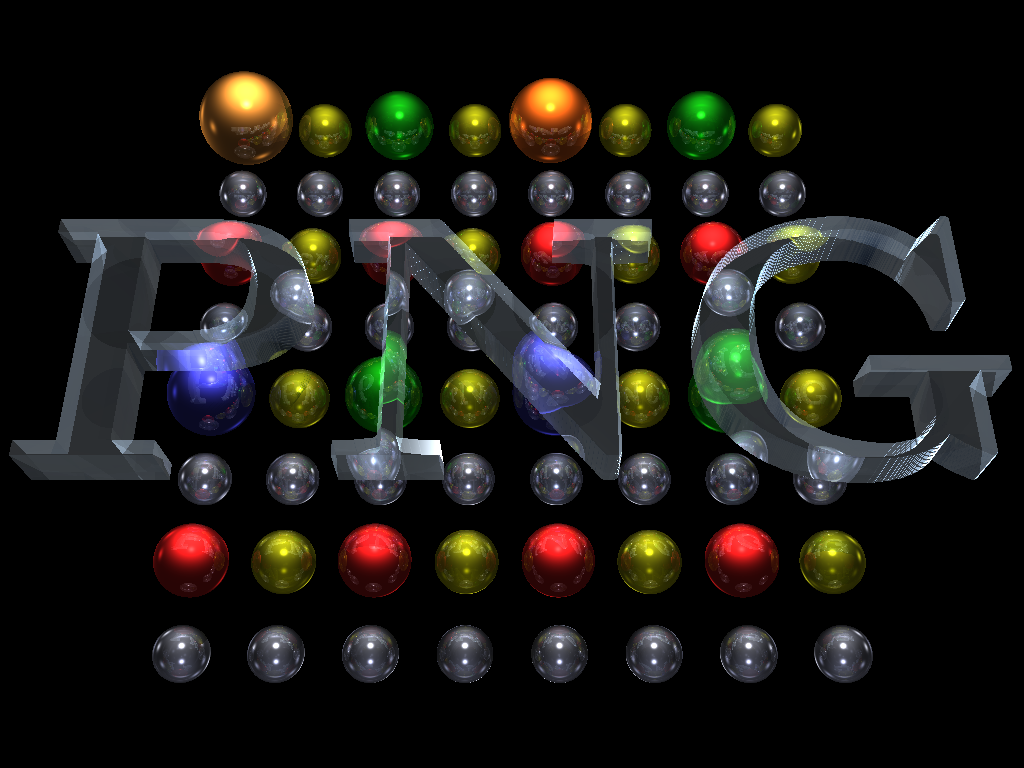
\includegraphics[width=0.30\textwidth]{images/pnglogo-blk.png}
    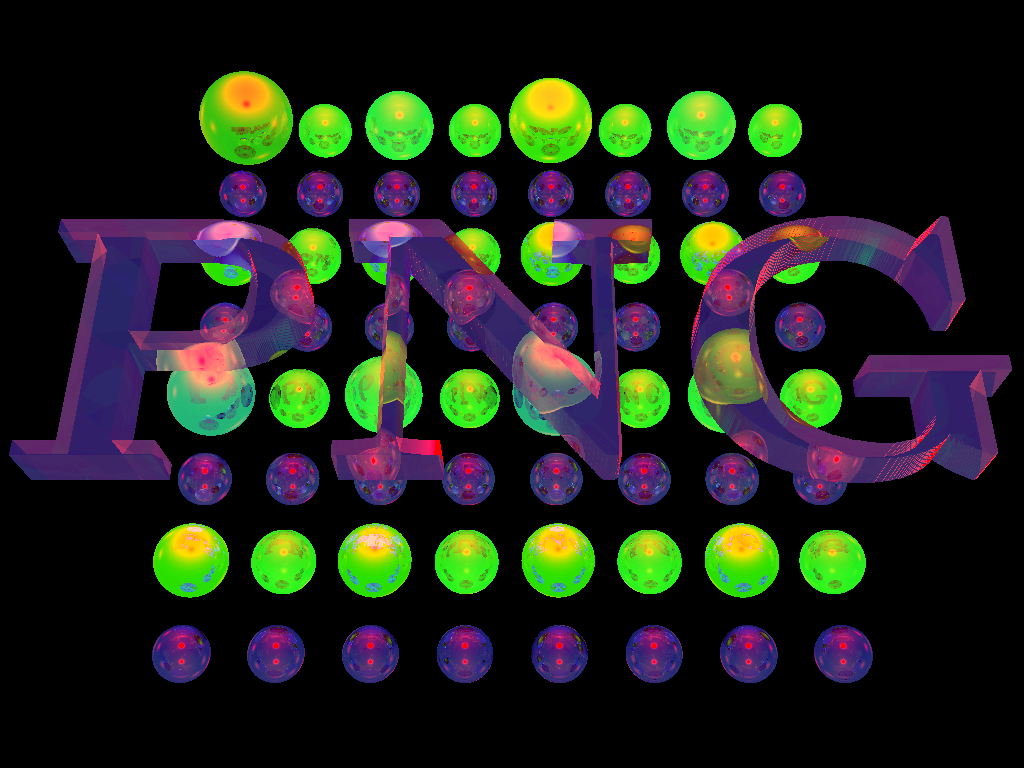
\includegraphics[width=0.30\textwidth]{images/results/hsv-cv.pnglogo-blk.png}
    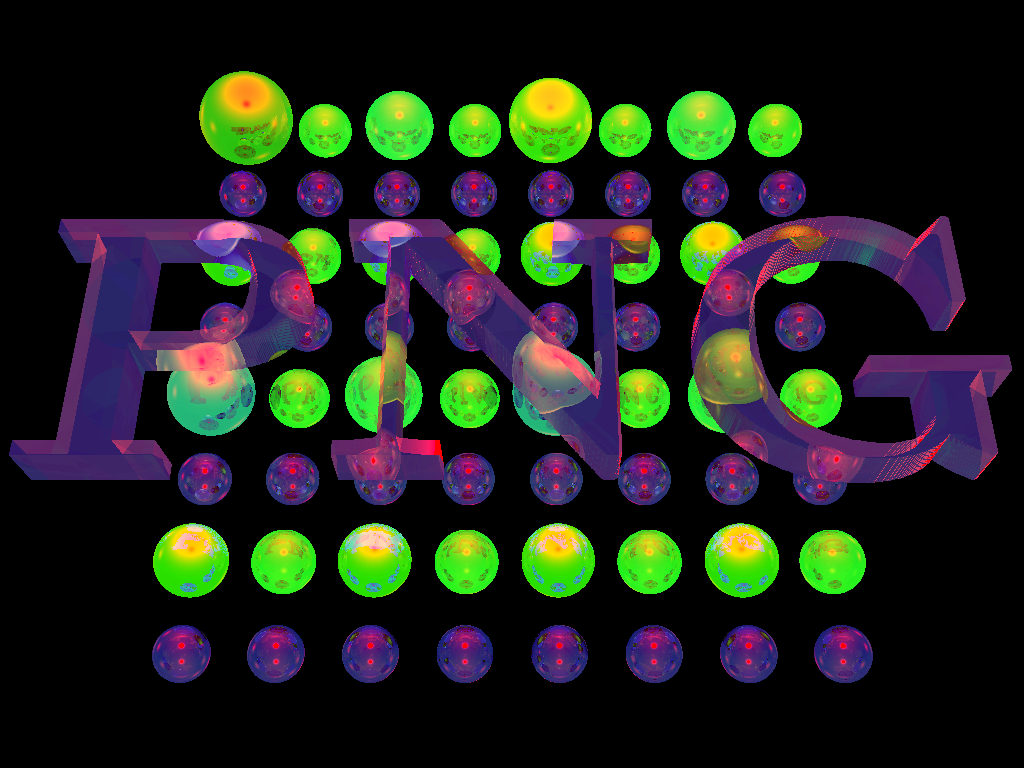
\includegraphics[width=0.30\textwidth]{images/results/hsv-my.pnglogo-blk.png}

    \begin{center}
        \caption{HSV results of OpenCV (middle) and self-implemented  Algorithm (right)}            
    \end{center}

    \label{fig:hsv1}
\end{figure}


The top performance results for HSV were $ 1.67335 $ ms, $ 26.5975 $ ms  and $ 2.78265 $ ms for the three images. In comparison OpenCV took $ 0.2243 $ ms, $ 1.29245 $ ms and $ 0.4109 $ ms.


\begin{center}
    \begin{figure}[H]
        \centering
        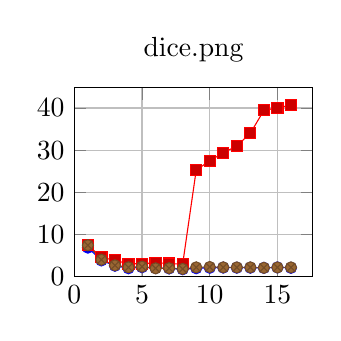
\begin{tikzpicture}
    \begin{axis}[
        title={dice.png},
        width=0.38\textwidth,
        xmin=0,
        ymin=0,
        grid=major
    ]
        \addplot coordinates {
            (1,6.8133)(2,3.772)(3,2.5074)(4,1.9063)(5,2.1592)(6,1.9498)(7,1.86735)(8,1.67335)(9,1.91465)(10,2.0285)(11,2.0644)(12,2.04225)(13,2.0411)(14,1.9984)(15,2.10485)(16,2.00745)
        };

        \addplot coordinates {
            (1,7.39955)(2,4.5312)(3,3.76235)(4,2.98635)(5,2.99115)(6,3.22585)(7,3.03185)(8,2.87065)(9,25.2141)(10,27.4829)(11,29.348)(12,30.9892)(13,34.0131)(14,39.4454)(15,40.0405)(16,40.7224)
        };

        \addplot coordinates {
            (1,7.38385)(2,3.9323)(3,2.60535)(4,2.11995)(5,2.28335)(6,1.88385)(7,1.92715)(8,1.75435)(9,2.12325)(10,2.2048)(11,2.12435)(12,2.10905)(13,2.11495)(14,2.00945)(15,2.1006)(16,2.1095)
        };
    \end{axis}
\end{tikzpicture}
%
%
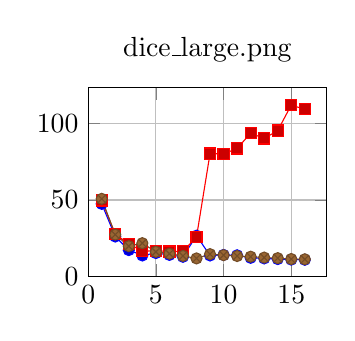
\begin{tikzpicture}
    \begin{axis}[
        title={dice\_large.png},
        width=0.38\textwidth,
        xmin=0,
        ymin=0,
        grid=major
    ]
        \addplot coordinates {
            (1,47.4856)(2,26.0906)(3,17.1762)(4,13.65)(5,15.2361)(6,14.0216)(7,12.7772)(8,26.5975)(9,13.65)(10,14.0004)(11,13.7465)(12,12.1108)(13,11.7167)(14,11.2901)(15,10.9296)(16,10.8207)
        };

        \addplot coordinates {
            (1,49.7317)(2,27.5263)(3,21.3296)(4,16.3962)(5,16.8052)(6,16.226)(7,16.3412)(8,25.7123)(9,80.4579)(10,80.2426)(11,83.8239)(12,93.8307)(13,90.3553)(14,95.5529)(15,112.304)(16,109.444)
        };

        \addplot coordinates {
            (1,50.772)(2,27.3163)(3,19.7423)(4,21.7001)(5,16.0099)(6,14.8033)(7,13.3408)(8,11.7108)(9,14.5207)(10,13.8433)(11,13.274)(12,12.845)(13,12.2565)(14,11.8881)(15,11.2955)(16,11.1468)
        };
    \end{axis}
\end{tikzpicture}
%
%
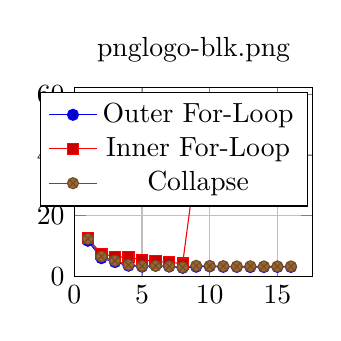
\begin{tikzpicture}
    \begin{axis}[
        title={pnglogo-blk.png},
        width=0.38\textwidth,
        xmin=0,
        ymin=0,
        grid=major
    ]
        \addplot coordinates {
            (1,11.7365)(2,5.97965)(3,4.69315)(4,3.49675)(5,3.18585)(6,3.52845)(7,3.20715)(8,2.78265)(9,3.15175)(10,3.2601)(11,3.12815)(12,3.10095)(13,3.05015)(14,3.06365)(15,3.08175)(16,3.07475)
        };
        \addlegendentry{Outer For-Loop}

        \addplot coordinates {
            (1,12.5315)(2,7.41705)(3,6.46785)(4,6.26345)(5,5.4006)(6,4.88325)(7,4.59995)(8,4.20975)(9,37.9699)(10,36.2843)(11,38.3156)(12,40.1812)(13,42.0504)(14,44.4038)(15,56.4891)(16,55.9547)
        };
        \addlegendentry{Inner For-Loop}       

        \addplot coordinates {
            (1,12.3462)(2,6.5227)(3,5.1136)(4,3.7885)(5,3.38175)(6,3.42255)(7,3.28445)(8,2.93785)(9,3.43565)(10,3.3931)(11,3.33495)(12,3.2319)(13,3.29275)(14,3.2345)(15,3.2412)(16,3.25085)
        };
        \addlegendentry{Collapse}
    \end{axis}
\end{tikzpicture}
        \caption{Performance results of HSV conversion algorithm}
    \end{figure}
\end{center}

\section{Emboss}

As OpenCV doesn't offer an implementation of the Emboss algorithm, no comparison was possible.

\begin{figure}[H]
    \centering

    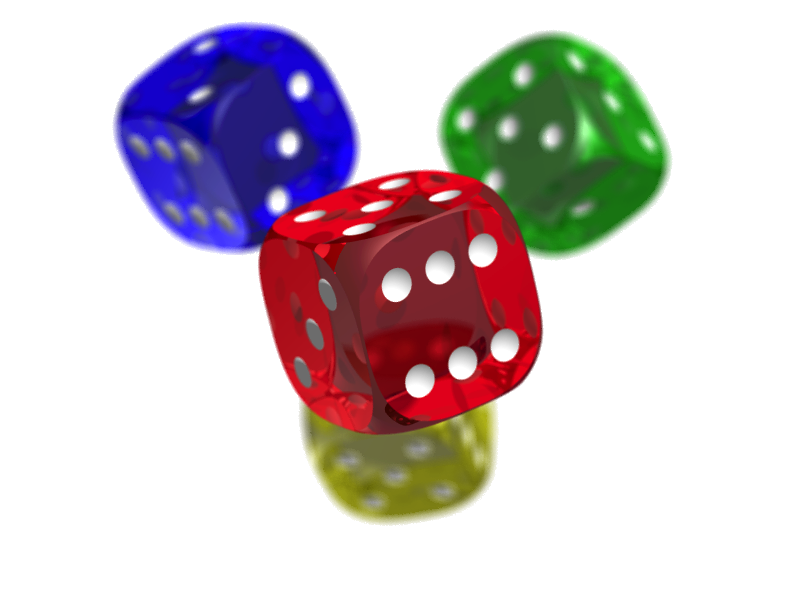
\includegraphics[width=0.30\textwidth]{images/dice.png}
    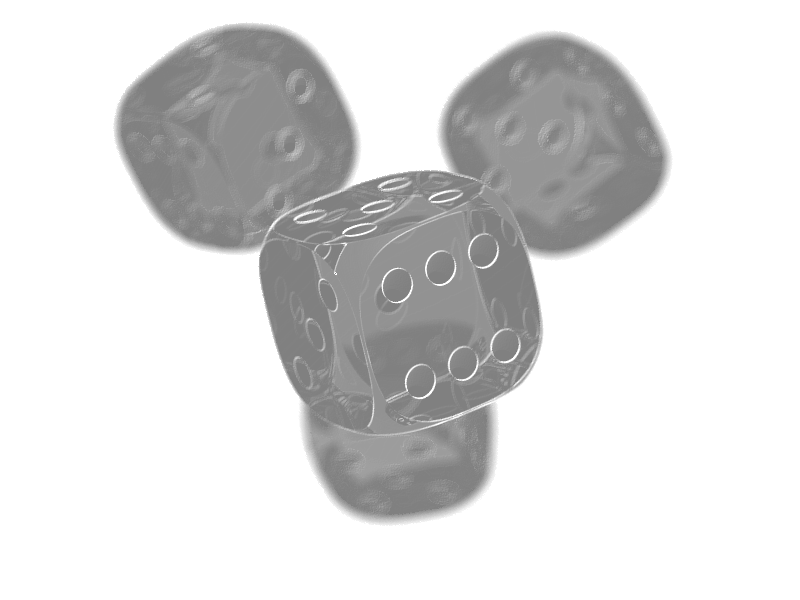
\includegraphics[width=0.30\textwidth]{images/results/emboss-my.dice.png}
    \\
    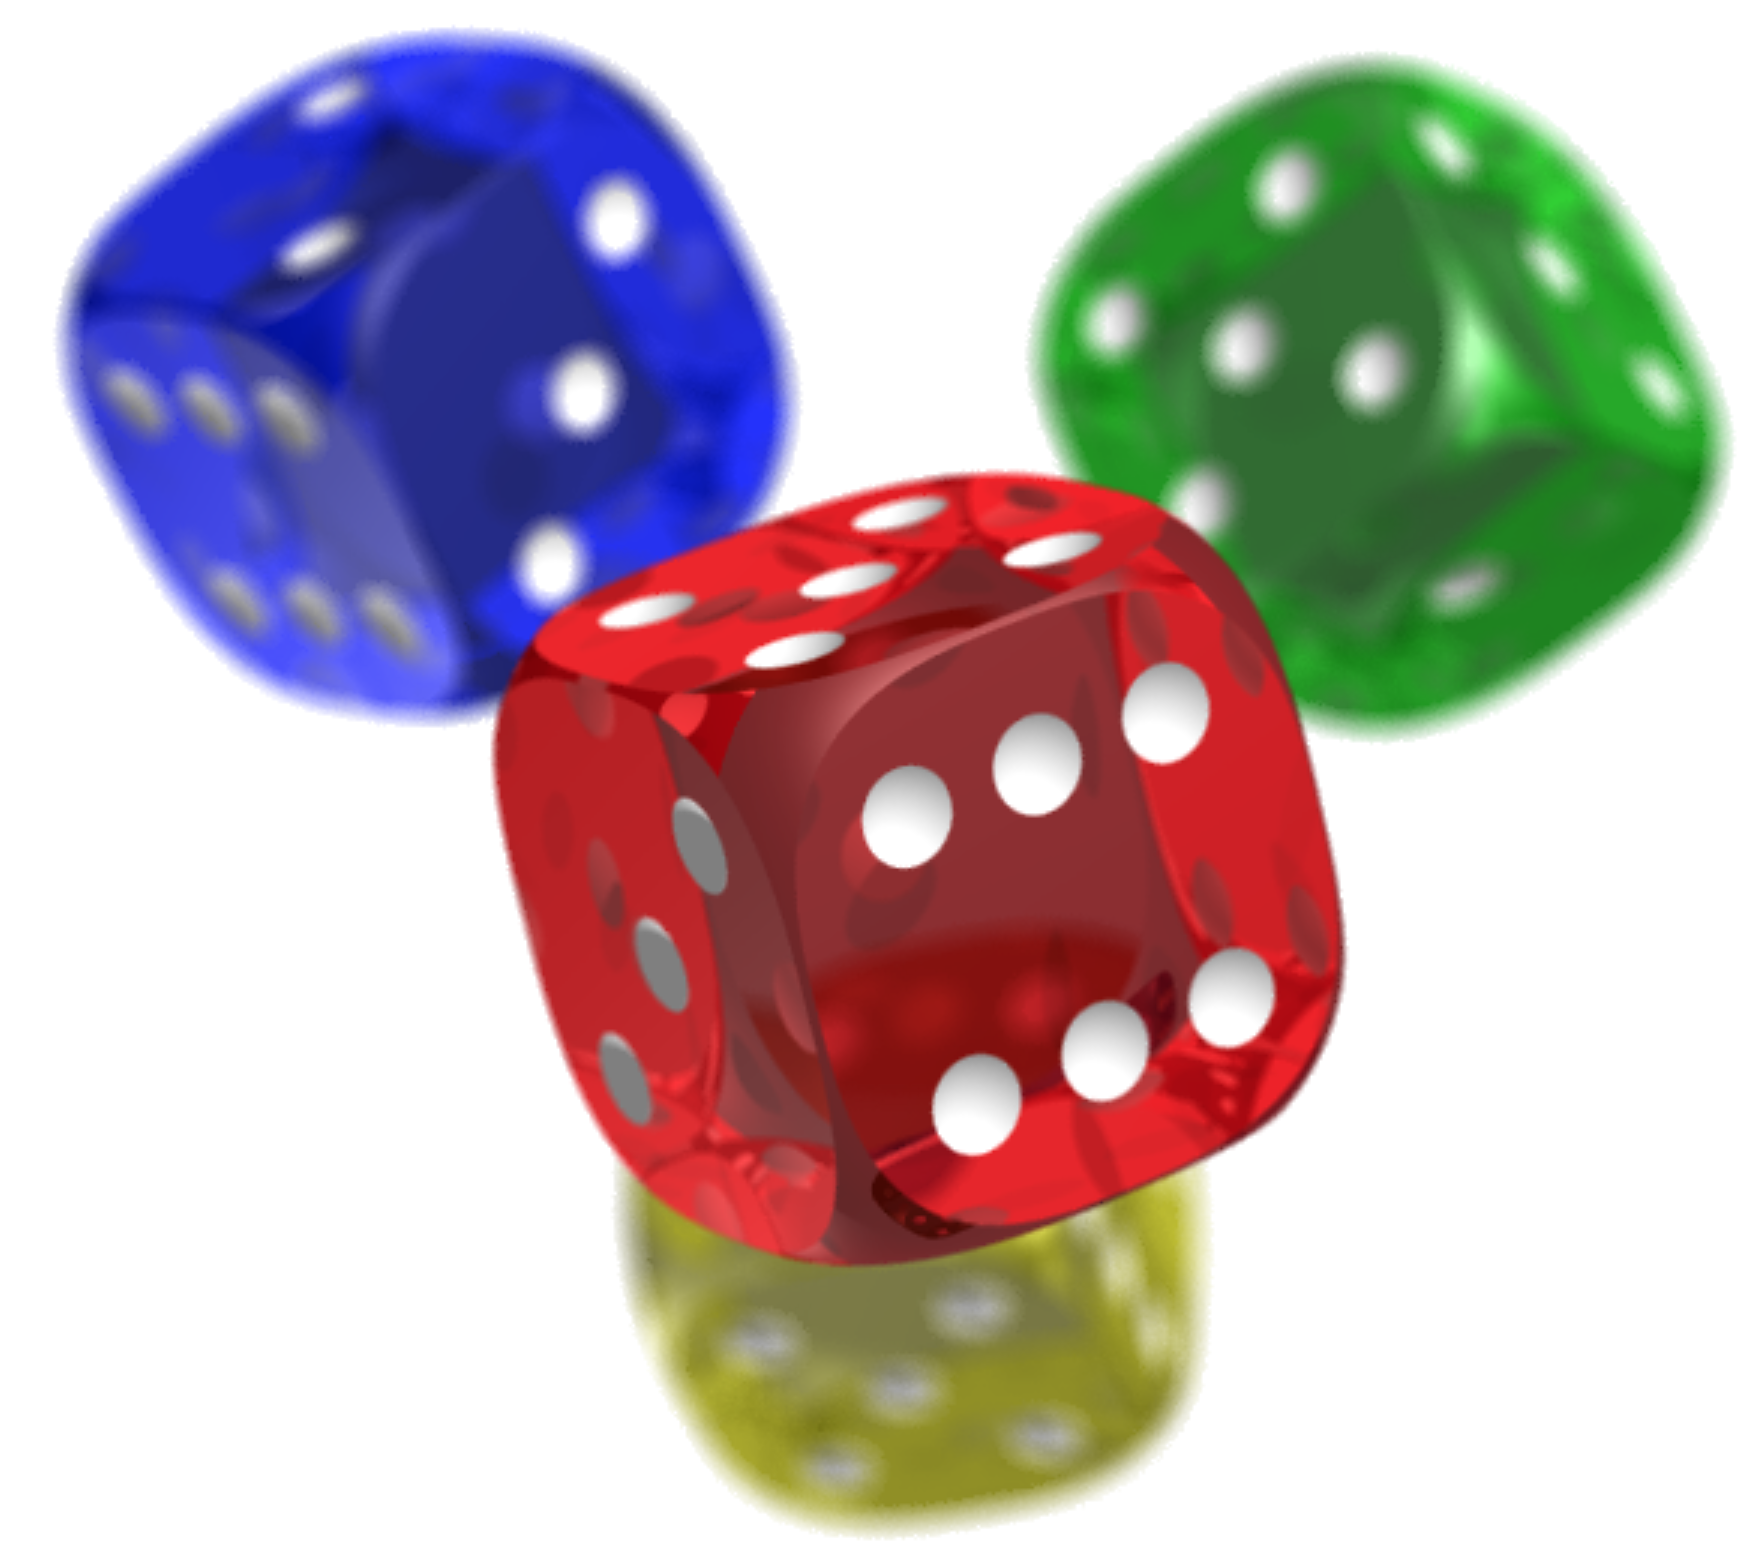
\includegraphics[width=0.30\textwidth]{images/dice_large.png}
    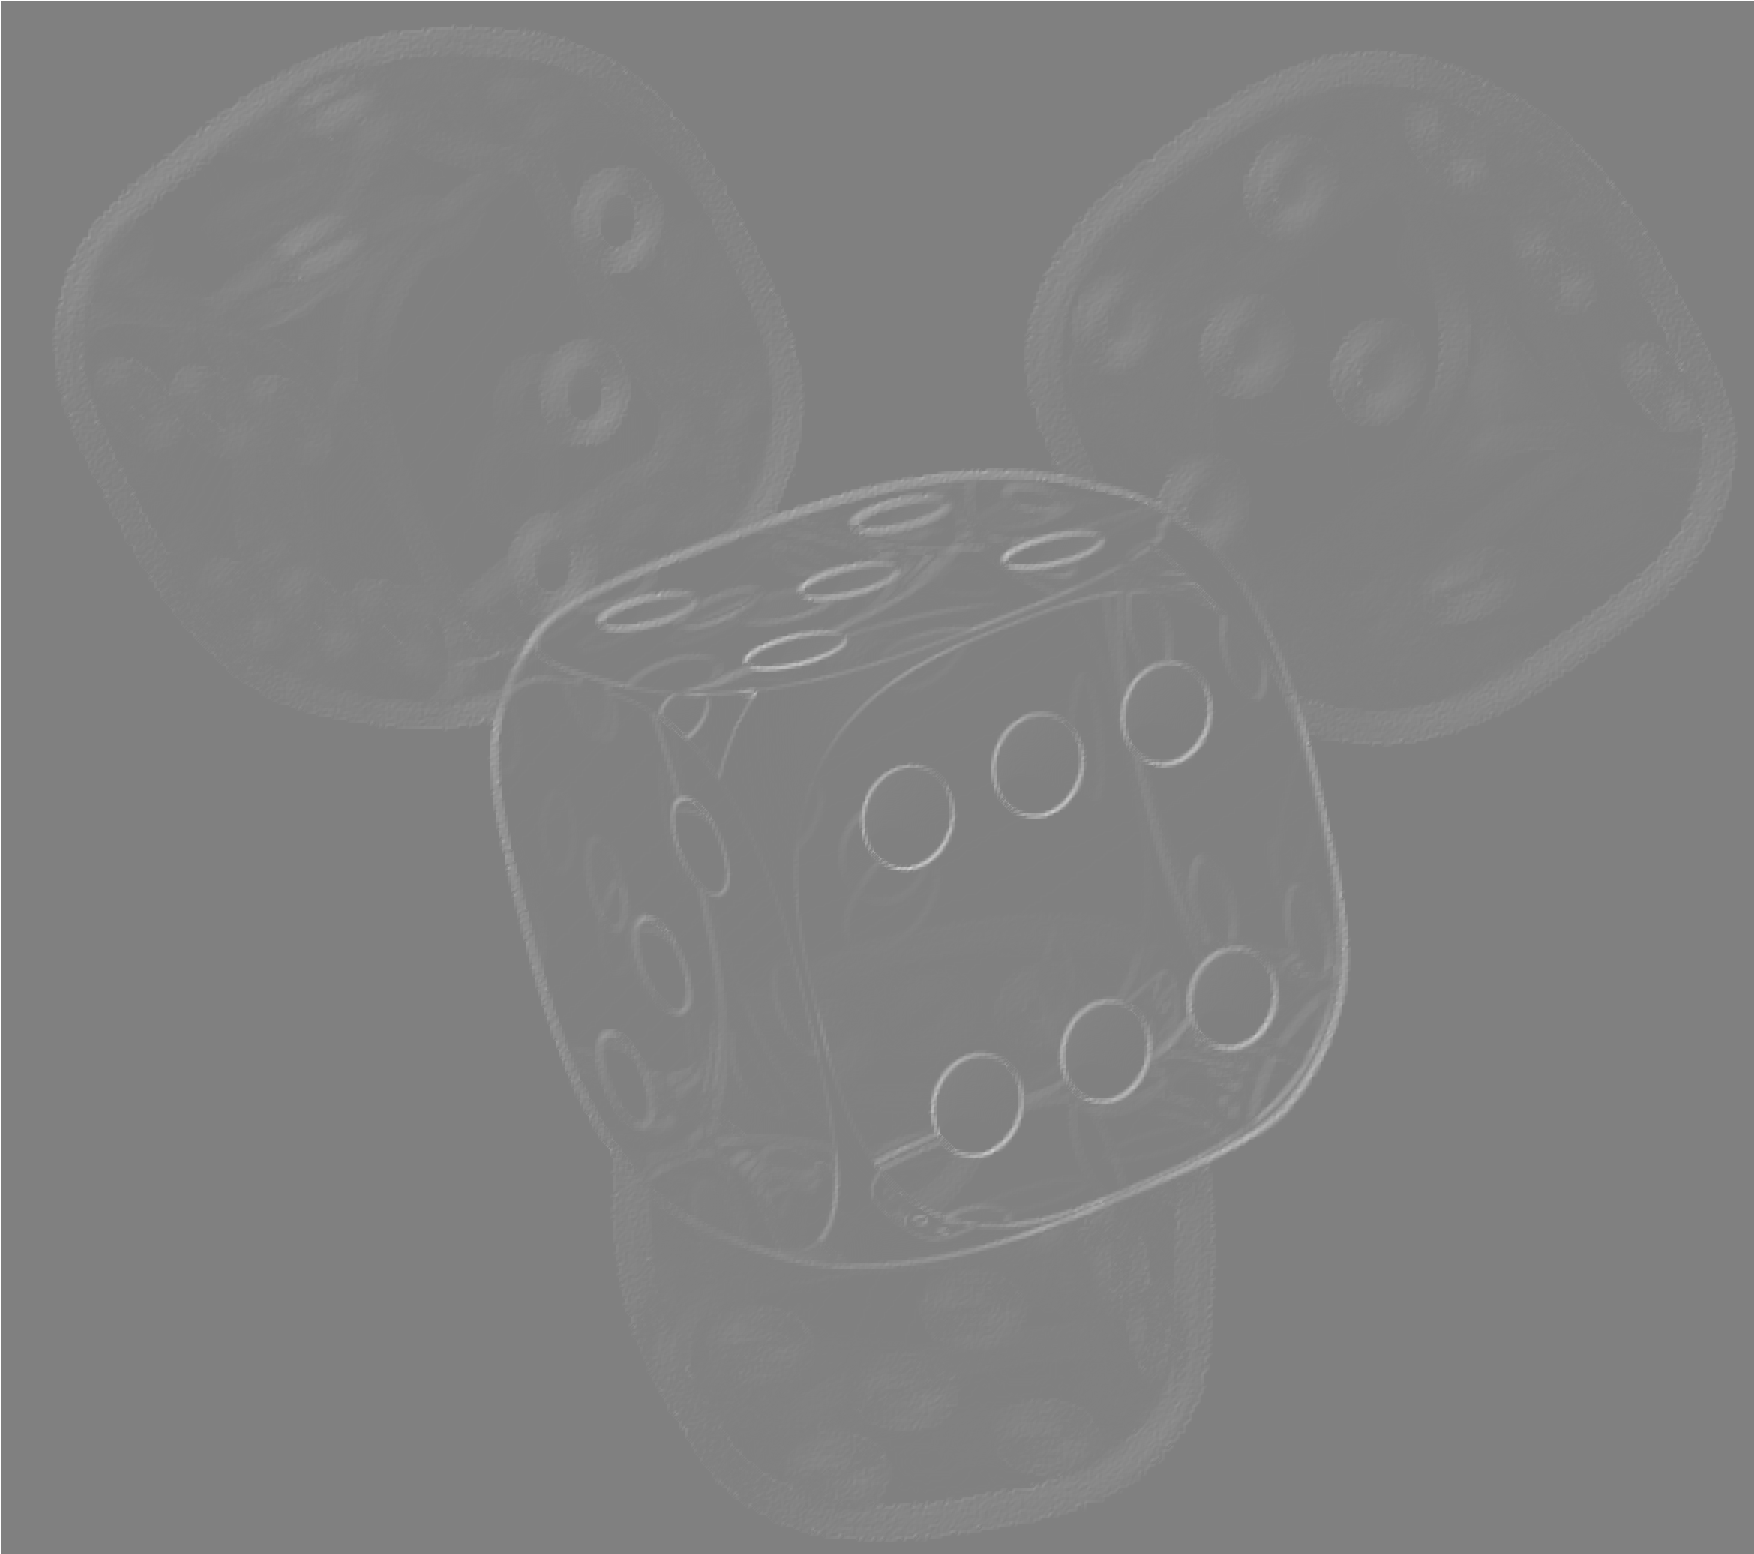
\includegraphics[width=0.30\textwidth]{images/results/emboss-my.dice_large.png}
    \\
    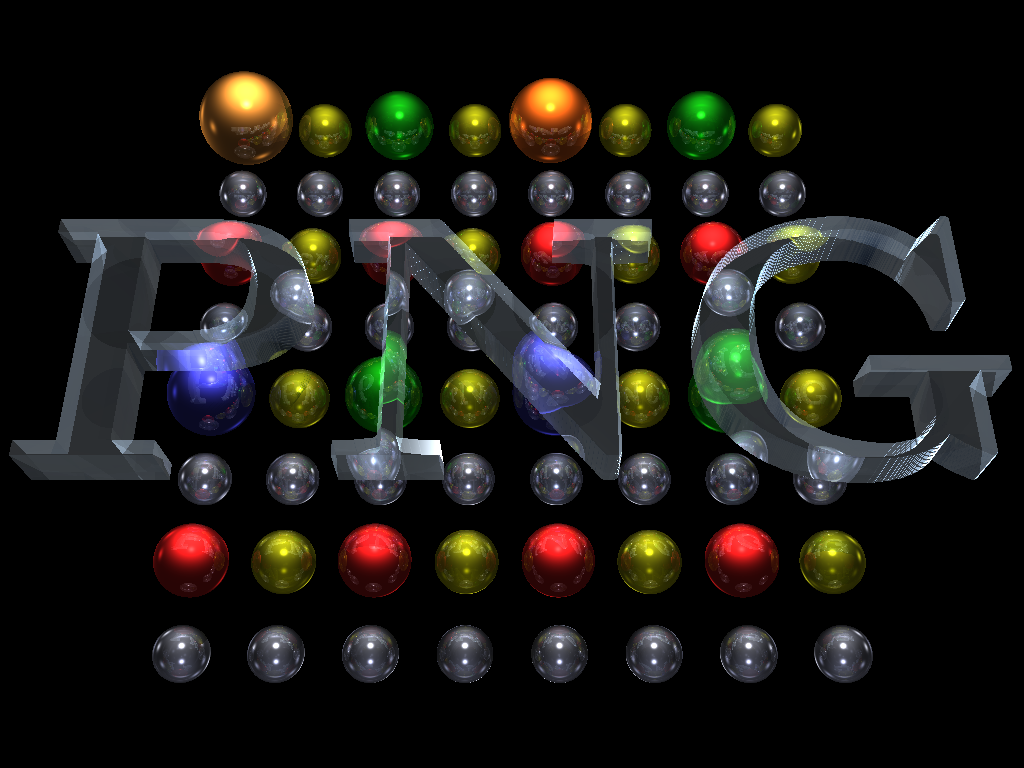
\includegraphics[width=0.30\textwidth]{images/pnglogo-blk.png}
    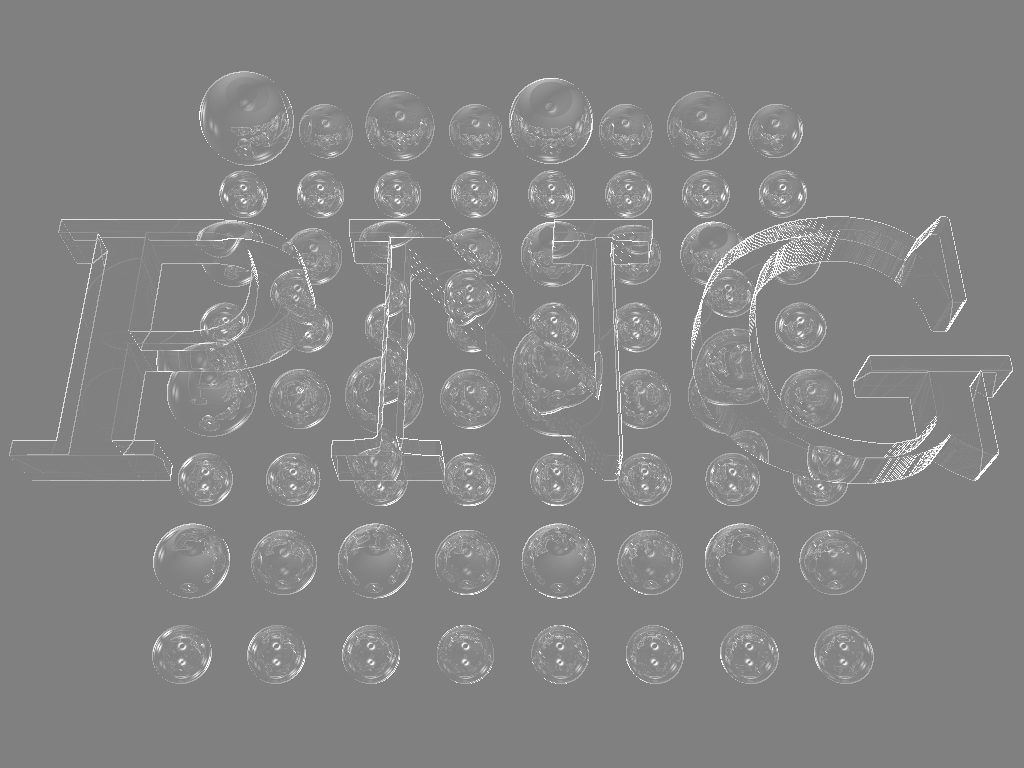
\includegraphics[width=0.30\textwidth]{images/results/emboss-my.pnglogo-blk.png}
    
    \begin{center}
        \caption{Emboss results of self-implemented Algorithm (right)}
    \end{center}

    \label{fig:emboss1}
\end{figure}

The top performance results for Emboss were $ 1.1699 $ ms, $ 6.6008 $ ms  and $ 1.90685 $ ms for the three images.

\begin{center}
    \begin{figure}[H]
        \centering
        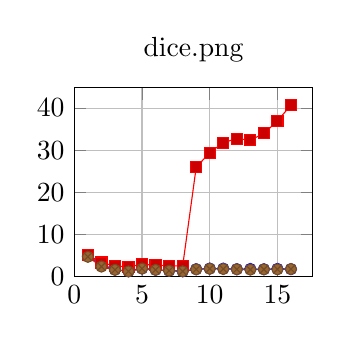
\begin{tikzpicture}
    \begin{axis}[
        title={dice.png},
        width=0.38\textwidth,
        xmin=0,
        ymin=0,
        grid=major
    ]
        \addplot coordinates {
            (1,4.8388)(2,2.8324)(3,1.59845)(4,1.19935)(5,1.87025)(6,1.56525)(7,1.34835)(8,1.1991)(9,1.68795)(10,1.8391)(11,1.81815)(12,1.6916)(13,1.7405)(14,1.67545)(15,1.7581)(16,1.701)
        };

        \addplot coordinates {
            (1,5.06275)(2,3.26365)(3,2.45605)(4,2.23675)(5,2.84175)(6,2.64125)(7,2.52415)(8,2.43215)(9,25.9095)(10,29.4058)(11,31.7735)(12,32.7392)(13,32.3443)(14,33.981)(15,36.9086)(16,40.7253)
        };

        \addplot coordinates {
            (1,4.6275)(2,2.3012)(3,1.5294)(4,1.153)(5,1.82735)(6,1.523)(7,1.31275)(8,1.1699)(9,1.64575)(10,1.7925)(11,1.73355)(12,1.65625)(13,1.58)(14,1.6422)(15,1.65035)(16,1.7164)
        };
    \end{axis}
\end{tikzpicture}
%
%
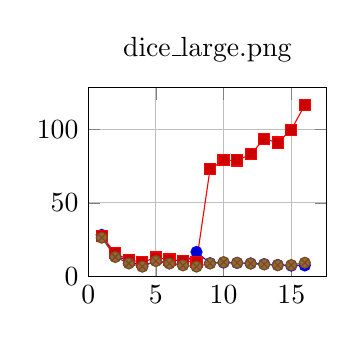
\begin{tikzpicture}
    \begin{axis}[
        title={dice\_large.png},
        width=0.38\textwidth,
        xmin=0,
        ymin=0,
        grid=major
    ]
        \addplot coordinates {
            (1,28.1787)(2,13.6684)(3,10.6587)(4,6.841)(5,10.6448)(6,8.9229)(7,7.7613)(8,16.5284)(9,8.8759)(10,9.3305)(11,9.0727)(12,8.75325)(13,8.265)(14,7.6939)(15,7.22555)(16,7.37725)
        };

        \addplot coordinates {
            (1,27.5487)(2,15.6059)(3,11.1323)(4,9.5563)(5,12.7669)(6,11.3685)(7,10.444)(8,9.8202)(9,72.9501)(10,78.8844)(11,78.8677)(12,82.9903)(13,93.5949)(14,91.0306)(15,99.7156)(16,116.585)
        };

        \addplot coordinates {
            (1,26.2787)(2,13.1285)(3,8.74935)(4,6.5788)(5,10.3955)(6,8.6642)(7,7.436)(8,6.6008)(9,8.76145)(10,9.5894)(11,9.1864)(12,8.6334)(13,8.10475)(14,7.5467)(15,7.62205)(16,9.2002)
        };
    \end{axis}
\end{tikzpicture}
%
%
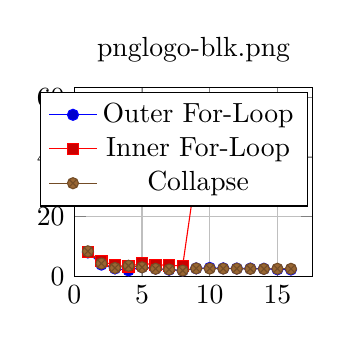
\begin{tikzpicture}
    \begin{axis}[
        title={pnglogo-blk.png},
        width=0.38\textwidth,
        xmin=0,
        ymin=0,
        grid=major
    ]
        \addplot coordinates {
            (1,7.98865)(2,3.91065)(3,2.608)(4,1.9658)(5,3.07375)(6,2.5663)(7,2.21405)(8,1.9445)(9,2.64595)(10,2.81395)(11,2.65795)(12,2.60165)(13,2.5888)(14,2.52365)(15,2.3272)(16,2.2523)
        };
        \addlegendentry{Outer For-Loop}

        \addplot coordinates {
            (1,8.1666)(2,4.98855)(3,3.6625)(4,3.2951)(5,4.29465)(6,3.90035)(7,3.6383)(8,3.53105)(9,35.0564)(10,37.7613)(11,40.0554)(12,39.6329)(13,41.5814)(14,43.8201)(15,47.1202)(16,57.4096)
        };
        \addlegendentry{Inner For-Loop}       

        \addplot coordinates {
            (1,8.37795)(2,4.27585)(3,2.78925)(4,3.53475)(5,3.008)(6,2.5163)(7,2.269)(8,1.90685)(9,2.64125)(10,2.5832)(11,2.57355)(12,2.55125)(13,2.493)(14,2.47165)(15,2.52675)(16,2.50055)
        };
        \addlegendentry{Collapse}
    \end{axis}
\end{tikzpicture}
        \caption{Performance results of Emboss algorithm}
    \end{figure}
\end{center}
